\documentclass{article}
\usepackage{graphicx} 
\usepackage{changepage}
\usepackage{rotating}
\usepackage{adjustbox}
\usepackage{appendix}
\usepackage{pdflscape}
\usepackage{float}
\usepackage{graphicx}
\usepackage{subcaption}
\usepackage{booktabs}
\usepackage{siunitx}
\setlength{\parindent}{0pt}
\setlength{\parskip}{\baselineskip} 
\usepackage{threeparttable}
\usepackage{setspace}
\usepackage[hidelinks]{hyperref}
\usepackage{tabularx} % in the preamble


\addtolength{\oddsidemargin}{-.5in}%
\addtolength{\evensidemargin}{-.5in}%
\addtolength{\textwidth}{1in}%
\addtolength{\textheight}{1.3in}%
\addtolength{\topmargin}{-.8in}%



\title{The London Laundromat: The Effects of Transparency on The London Offshore Property Market}
\author{
By B171234 \\
\vspace{1cm}
Word Count: [9885] }
\date{April 2024}


\begin{document}
\maketitle
\setstretch{1.5}

\begin{abstract}
Following the Russian invasion of Ukraine in February 2022, investigative reports have revealed the scale of corruption and money laundering rooted in the London property market. In this study, I measure the impact of the Economic Crime Bill (ECB), which marks the attempt made by the UK government to introduce greater transparency and expose the anonymous ownership of property. Taking advantage of data on property transactions made by overseas companies, I show that the implementation of the ECB has had a marginal effect in altering the investment behaviours of various stakeholders based in overseas territories in the short run. I also do not find any strong evidence of long-run behavioural alternations following the policy introduction. This research underscores the limitations of current legislative measures in addressing opaque ownership structures. It highlights the need for stronger enforcement and political accountability to combat the exploitation within the London property market.
\end{abstract}

\renewcommand{\abstractname}{Acknowledgements}
\begin{abstract}
I would like to thank Dr Georgios Manalis for his guidance and insightful contributions to the discussions in our meetings throughout the process of researching and writing this paper. 
\end{abstract}


\newpage 
\tableofcontents 
\newpage
\maketitle

\setstretch{1.5}
\normalsize

\section{Introduction}

Real estate has traditionally been a discreet haven for wealth, often obscuring the lines between legitimate investment and the concealment of illicit funds. In high-value property markets such as London, this secrecy has raised concerns about the ease with which money laundering can infiltrate the system, a phenomenon highlighted by the existence of tours showcasing properties owned by kleptocrats (Borisovich 2016). The attraction for real estate stems, in part, from its comparative lack of transparency, particularly against the backdrop of more regulated sectors such as banking (Bomare and Herry 2022). In this setting, real estate agents and others in the process of real estate transactions have not always been obligated to perform stringent background checks, especially when transactions involve offshore shell companies situated in tax havens. 

The conventional solution to this lack of transparency has been the introduction of beneficial owner transparency, mandating the revelation of ultimate owners to either the government or the public. However, empirical evidence, such as the study by Collin et al. (2021), questions the effectiveness of these measures, suggesting that while policy implementation is crucial, it alone may not be sufficient to stem illicit financial flows. Against this complex backdrop, this dissertation investigates the recent legislative effort by the UK government, the Economic Crime Bill (ECB), which in response to Russia's invasion of Ukraine in 2022, sought to reveal secrecy surrounding property ownership. With the establishment of a public Register of Overseas Entities, the ECB aimed to map offshore companies to the real estate they own within the UK, offering a new tool in the fight against economic crime. By using the data on land ownership and overseas company registration, this study employs a difference-in-differences design to evaluate the impact of the ECB on property purchases and sales by companies based in selected overseas jurisdictions.

This dissertation examines the impact of the UK's Economic Crime Bill on offshore property ownership in London's market. It begins with an introduction that presents the problem of money laundering through property investment and the legislative response. The literature review that follows addresses the problem in an academic context, exploring existing research on beneficial ownership transparency and foreign property ownership. The following sections will then proceed by presenting the methodology, detailing the empirical approach taken to assess the policy's impact, using a difference-in-differences analysis of ownership patterns. The results are then presented and discussed, highlighting why the results deviate from the existing literature and some of the limitations in our empirical approach. The dissertation concludes by reflecting on the findings, and their implications for policymakers and suggesting potential avenues for future research, offering a narrative from the initial hypothesis to conclusions.


\section{Background and Analytical Framework}
\subsection{London Laundromat}
London has been known as the world's capital for dirty money for many years. The city has become a hub for financial flows from illicit sources worldwide, including Russian assets worth nearly a billion pounds in London's residential property (Transparency International UK, 2022a). This can be traced back to the former British and Soviet empires. After the fall of the British Empire, many of its former dependencies needed a new purpose, which they found in providing financial secrecy and corporate camouflage to many individuals and corporations. This created a means for individuals to navigate through the increasingly globalised economy, allowing illicit money to flow within the UK (Financial Times, 2022). While Britain was establishing these overseas jurisdictions, the Soviet Union was on the verge of collapse. The scramble for the vast amount of wealth stored under the former regime created a Russian kleptocracy. A system that is characterised by a network of ruling elites that steal public funds for their private gain using public institutions (Mayne, 2022). Ultimately, this led to the creation of a new social class of ruling elite in Russia known as the Oligarchs.

Illicit wealth was able to filter into London as the financial sector became increasingly liberalised under the Thatcher regime. This pattern continued under subsequent governments, and for decades, the UK welcomed Russian money, regardless of where it was sourced. Boris Johnson, the former mayor of London, expressed a desire for the city to become the hub for Russian money, with the London Stock Exchange welcoming Russian companies (Financial Times 2022). The Labour government's 2008 Golden Visa scheme was perhaps the height of government anti-corruption myopia, introduced to bring wealth and capital into London (Wallis, 2023). However, the system was abused by oligarchs and kleptocrats to buy UK citizenship, which would rubber-stamp the legitimacy of their activities within the UK.

Integrating illicit wealth into the economy involves four key stages: Placement, Layering, Integration, and Defence. In the first stage, money is transferred from overseas accounts into the UK through shell companies that are typically registered in overseas jurisdictions. In the second stage, the money is moved around in complicated financial transactions to create a distance between the individual and the money's source. The third stage involves moving the money through various foreign territories before finally entering the UK. To establish this wealth in the UK financial system, the money is used to purchase assets, particularly UK property. Once the money enters the system, the user can use it at their discretion (Financial Times 2022).

A typical example of this is Roman Abramovich's £90 million mansion in Kensington Palace (Brennan, 2013). This is a general reflection of grade one/two listed properties purchased in high-end locations such as Belgravia, Knightsbridge, and Mayfair. In total, 84,000 homes in the UK are owned anonymously, valued at around £6.7 billion. Of this value, £1.5 billion is linked to Russians accused of corruption and those who have close links to the Kremlin, and £834 million is the estimated worth of property bought by Russians through the use of shell companies based in crowned dependencies (Transparency International UK 2022a). The final stage is defending the wealth accumulated. London's libel laws provide the perfect setting for these individuals to defend themselves from external threats to wealth. London has some of the top law firms and financial institutions in the world, creating an extensive network of intermediaries that ultimately provide the stamp of legitimacy to the reputation and wealth of kleptocrats and oligarchs.



\subsection{The 2022 Economic Crime Act and The Register of Overseas Entities}
In response to growing concerns about corruption in the UK, the government made efforts to deter illicit activity. In 2016, then-Prime Minister David Cameron proposed a measure during the Anti-Corruption Summit to address these issues and enhance transparency. Cameron suggested a registry of beneficial ownership that would include all overseas firms owning property in the UK, to deter exploitation within the real estate sector. However, after David Cameron's resignation as Prime Minister, subsequent conservative leaders deprioritised the initiative aimed at tackling illicit money within the UK economy. Individuals such as Lord Theodore Agnew, the UK Minister for Efficiency and Transformation, resigned in response to the government's stalling on the reform (Makortoff 2022). In response, Prime Minister Boris Johnson confirmed on February 2, 2022, that the bill would be put to a vote in the third-party parliamentary session of 2022 (Collin et al. 2023).

On February 24th, 2022, the Russian invasion of Ukraine brought to light the extent of illicit activities involving various Russian oligarchs within the UK. As political tensions escalated, taking a stricter approach towards Putin's allies was seen as a way to deter further aggression in Ukraine. Consequently, there was a push to expedite the implementation of the Economic Crime Bill (ECB). It was introduced into parliament on March 1st and received royal assent just two weeks later, becoming the Economic Crime Act (ECA) (Pickard, 2022).

A key aspect of the policy was the Register of Overseas Entities, which mandated that all foreign companies owning land in the UK disclose the identities of their beneficial owner(s). For any overseas firms that already owned properties or acquired new ones before August 1, 2022, a transitional period was established. These companies were given until January 31, 2023, to provide the necessary information on beneficial ownership to the register. The new law also stipulated that any overseas firm seeking to sell a property it already owned after February 28, 2022, must register with Companies House. Failure to register would prohibit the sale of the property. From then on, all foreign companies that purchased UK property would have to submit beneficial ownership information to the register to obtain legal title from the UK land registry (Collin et al. 2023). The registry was made live and publically available on August 1st.

Although the attempted transparency policy was seen as a significant step forward, serious concerns emerged regarding the effectiveness of the legislation in making a real impact. Investigative reports revealed issues in the existing Companies House registries, such as individuals using fake identities to register companies to a significant number of companies refusing to file reports altogether (Global Witness 2013; Williams 2022). The ECB was also flawed in that companies simply denied having any qualifying beneficial owners and directors (Transparency International UK). It was also problematic that companies could report nominee owners and directors, rather than true beneficial owners (Beioley et al. 2022). In addition, verifying ownership requires extensive resources, something that the UK government doesn't have in relative abundance given that it spends only 0.042\% of GDP on tackling economic crime, compared to the estimated £100 billion excess in economic crime per year (The Economist 2022). Examplafying the point is that the cost of registering a company through Companies House is completely inexpensive, costing £12, which ultimately limits the agency's ability to fund any preventative measures to ensure the accuracy of the reports (Hawley 2022).  

\subsection{Russian Informal Politics}
In the paper from Oligarchs to Oligarchy, Siegel, D. (2022) puts forward the idea that Russia’s Oligarchs act cohesively, particularly when their wealth is threatened from outside their resided country. The paper addresses the idea that Russia is best characterised by an oligarchy, with evidence showing that major players in Russia’s informal network have responded to U.S. sanctions by coalescing behind Putin. Consequently, recent developments in US foreign policy have now been formulated around the principle of Russia’s informal politics. A “patronal” system that extends beyond politics, penetrating all levels of society through countless intermediaries (Henry Hale 2015, 9-10).  U.S. sanctions assume that Russia’s informal politics makes it uniquely vulnerable, targeting sanctions on Oligarchs and individuals with close ties to Putin seems a clever way to exert meaningful political pressure on state leaders. However, what is evident following Russia’s invasion of Crimea in 2014, is that we observe an increasingly more belligerent and aggressive response after sanctions were imposed. The fact that this pattern continued to Russia's invasion of Ukraine, is evidence that sanctions have not succeeded in reversing Russia’s first move or deterring subsequent ones (Siegel, D. 2022).  

Fundamentally, rather than destabilising Putin’s rule through internal battles between oligarchs. U.S. sanctions might be the unifying force in Russia’s informal politics, creating a more coherent social class with the common interest of defending their wealth against Western hegemony. In this paper, I will extend this analysis to a policy introduced by the UK government. Specifically, the Economic Crime Bill (ECB) was established in response to Russia’s invasion of Ukraine and the subsequent exposure of Russia's illicit wealth held in the UK property market. Crucially, this policy draws parallels to the foundational elements of the sanctions imposed by the United States, concerning destabilising certain individuals. Although it is a universal policy that aims to deter all illicit actors; the ECB is a policy that implicitly threatens the wealth of oligarchs who hold wealth within property in London, rather than specifically attempting to attack the Russian economy. Whether we observe cohesive behaviour within the offshore property market by Russian nationals is difficult to quantify, given the limited data available on true beneficial ownership. However, the theoretical basis of Russian informal politics is useful in attempting to explain the findings of this paper. Therefore, this will form the foundational basis of our discussion and baseline criteria to assess the general impact of the ECB.


\subsection{Methodology and Expectations}
Our focus in this paper is to assess how increased transparency affects the investment of Russian nationals in London property. To achieve this, we will analyse the impact of the Economic Crime Bill, a policy aimed at promoting transparency, which was reintroduced after the Russian invasion of Ukraine in February 2022. In addition, we will refer to the theoretical framework proposed by Siegel, D. (2022) to evaluate and explain the results.

As it is not possible to directly identify Russian investors, I will observe their behavioural patterns concerning their use of overseas jurisdictions classified as havens. Therefore, to measure changes in Russian property investment, I will examine changes in the ownership of property owned by companies registered in these overseas jurisdictions. To then formulate the analysis, I will group these havens based on their favourability by Russians. Importantly, I will use a difference-in-difference approach to measure the effect of the ECB. The first treatment group will be the havens favoured by Russians.  And then expanding the analysis by categorising overseas buyers based on their use of certain havens to formulate additional treatment groups to capture the universal effect of the policy. Overall, any causal effect following the introduction of the policy would be characterised by changes in property ownership by overseas companies registered in these overseas jurisdictions, especially for groups of individuals who have an incentive to conceal their true ownership. A decline in the number of properties owned by these overseas companies would indicate that the policy has been effective in exposing beneficial ownership, at least in the short run.

It is important to acknowledge that categorising certain groups based on their use of overseas jurisdictions has some limitations. Therefore, in addition to classifying Russian beneficial ownership based on their use of havens, I will try to enhance the accuracy of this measurement by considering additional behavioural traits, particularly their tendency to own property in certain London districts. To achieve this, I am modelling this additional characteristic in a triple difference-in-difference framework. This alternative approach should theoretically enhance the accuracy of our attempt to identify true Russian beneficial ownership and the effects of transparency in Russian property ownership.


\section{Related Literature}
\subsection{Beneficial Ownership Transparency}
This dissertation relates to several important themes to the empirical literature on beneficial ownership transparency, and efforts to reduce illicit financial flows within the UK. Drawing parallels with Collin, M. , Hollenbach, F.M., Szakonyi, D. (2023) working paper as one of the first evaluations of a policy implemented to counter money laundering by increasing transparency within a single property market. Their framework forms the foundation of my empirical model. Extending on their methodology, I construct a difference in difference framework to observe the impact following the introduction of the ECB. However, in adopting the classification of Russian nationals by their use of havens, I attempt to improve the accuracy with regards to identifying true beneficial ownership by taking into account additional agglomeration behaviour. Specifically, observing the investment behaviour of Russians within certain districts in London. Crucially, this paper aligns with certain conclusions drawn by Collin, M. , Hollenbach, F.M., Szakonyi, D. (2023). With regards to the short-term effectiveness of the ECB is largely attributed to the public availability of the beneficial ownership registry. In contrast to the author's previous findings that evaluated the impact of Geographic Targeting Orders (GTOs) introduced in the United States. Finding that because GTOs kept information with regards to beneficial ownership behind closed doors, the result had little to no deterrent effect on illicit activities by shell companies. 

Additionally, this dissertation contributes to the literature on how policies that attempt to uncover ultimate ownership can lead to changes in illicit wealth from specific markets. This includes the research that measures the adverse impact transparency initiatives have had on different types of offshore wealth (Beer et al. 2019; Casi et al 2020; Menkhoff and Miethe 2019: O’Reilly et al. 2019). In addition, various studies that document the increased risk associated with non-compliance to financial regulation lead to the subsequent alteration in their behaviour (Londono-Velez and Avila-Mahecha 2021; Bethman and Kvasnicka 2016).

\subsection{Foreign Property Ownership}

This paper is also an addition to the work documenting the stock of foreign-owned property in heterogeneous markets. Alstadseater et al. (2022) examines the extent of foreign investment in Dubai's real estate market- finding that geographic proximity and historical ties are the leading factors to the 146 billion invested from conflict-afflicted countries and autocracies. Cvijanovic and Spaenjers (2021) observe the impact of non-resident foreign investment in the Paris housing market and find socioeconomic status driving up demand in desirable neighbourhoods. Further seminal papers by Alstadsæter (2022) and De Simone (2015); Sá (2016) also explore these themes within the Norwegian and UK property markets, respectively. 

Bomare and Herry (2022) serve as an important point of analysis in this dissertation. The authors investigate how the introduction of the Common Reporting Standard (CRS); which introduced cross-border reporting requirements for financial assets, but not real estate assets, had affected real estate investments in the United Kingdom. Grouping tax havens by their exposure to the countries that committed to introducing the CRS. Finding that the introduction of the CRS caused an increase in Real estate investments via tax havens exposed to the CRS. I will therefore use their findings to include CRS participating countries to formulate one of the treatment groups in my analysis, in doing so this will allow us to estimate whether any changes in offshore ownership are being driven by tax evasion efforts. 


Finally, as previously mentioned, I will build upon the body of literature concerning the impact of foreign policy formalised upon the theories of informal politics. While previous work by Seigal (2019); Henry Hale (2015) have addressed the wider discussion on Russian informal politics, this paper will attempt to expand and quantify the theoretical explanations, using the London property market as a case study for this.

\section{The Data}
\subsection{London Offshore Market}
London has commonly been an attraction for international real estate investments, specifically from those that feature at the top of the wealth distribution (Knite Franck, 2016). Because of this average property prices within London have been increasing since the beginning of the 2000s (Sá, 2016). 

This paper focuses on a particular area of the property market in the UK, which is commonly referred to as the offshore real estate market- properties that are owned by companies incorporated in jurisdictions outside of the United Kingdom. It is important to note that this form of ownership is not completely illegal. Some of these investments made by an offshore intermediary are used for legitimate purposes (Bomare and Herry 2022). However, the use of a shell company is typically favoured for illicit financial purposes because it allows individuals to keep their true identities hidden. Such that it is easier for the actual individual or corporation to not report the ownership of the property to the tax administration of their home country, but it is also a means of filtering and legitimising dirty money into the economy. 

Nonetheless, the owners of shell companies still must comply with taxes used in the UK. Four main taxes apply to owners of UK property: Land Tax and Stamp duty when purchasing a property, Capital Gains Tax when selling the property, Income Tax if the property generates an amount of rental income and Inheritance tax. UK residents and non-UK residents have been able to limit their liabilities concerning these taxes by essentially enveloping UK properties with an offshore company (Bomare and Herry 2022). It wasn’t until 2012 onwards that the UK government started to enforce tax changes to reduce the advantages formerly benefiting owners of enveloped properties within the UK. Regardless of this, illicit actors still benefited from being able to store vast amounts of wealth within this form of asset. That enables the discretionary spending and circulation of dirty money in the UK.

\subsection{The Overseas Companies Ownership Dataset (OCOD)}
To capture the stock, purchase and sale of UK property, I use the Overseas Companies Ownership Dataset (OCOD), which is publicly available on the UK land registry. It documents all real estate transactions made in England and Wales by companies registered outside the UK and has been updated monthly since 2015. The dataset provides information on the time and location of when the property was purchased, the price paid, the tenure of the property, and information on the purchasing company. To capture monthly changes in transactions of properties between various jurisdictions, I aggregate each monthly updated version of the dataset from January 2021 to February 2024 based on the title number and the country where the company is incorporated. To focus solely on transactional behaviour within the London property market, I filter the aggregated data accordingly.

It is important to note that the OCOD has certain limitations that need to be taken into account during data analysis. One of the main challenges is that some addresses are recorded as free text, which can be incomplete and contain 'nested' properties. It means that if a single company buys multiple properties at the same time, it is recorded as a single unique transaction within the registry (Bomare and Herry 2022). For example, in my sample, there is an entry \textit{"168, 170, 172, 176, 178, 180 and 182 Portobello Road, London (W11 2EB)"}, that contains multiple properties in a single row. To address this issue, a series of data parsing would be needed to separate each property as its entry within the registry to improve the validity of estimates (Bourne et al. 2023). However, due to time constraints and the large sample size of over 1.5 million data points, I was unable to perform this data processing. Nonetheless, given the large sample size, a general effect can still be captured.

In addition to OCOD, there is also the UK Companies that Own Property in England and Wales (CCOD) dataset. It contains information on all properties bought by companies registered in the UK since March 2014. If we consider these two datasets in combination, they only contain information regarding transactions of overseas and domestic companies, not other entities. For instance, if an overseas company sells a property to an individual, the transaction is documented in OCOD with information on the seller, but the dataset does not contain information on the actual individual. Similarly, if a domestic company within the UK sells a property to an overseas company, then the sale is registered in the CCOD registry, and the purchase is documented in the OCOD registry (Collin et al. 2023). For this paper, I am primarily focused on the change in properties from overseas companies and will focus on the transactions within the OCOD dataset. Therefore the purchase and sale of property could be made to and from either another overseas company, a UK domestic company or an individual(s). 

\subsection{Identifying and classifying Jurisdictions Favoured by Certain Groups}
To identify jurisdictions that are favoured by different groups. I will draw upon the identified havens used by Collin et al. (2023). I do this firstly because there is restricted access to certain offshore leaked data files such as the OpenLux and CNBIOM data, and secondly, many of the entities identified in the available leaked datasets, have many unclassified results to exposed entities that are associated with certain countries. Creating a skewed classification of jurisdictions associated with certain groups. Particularly when attempting to identify Russian-favoured havens, many of the jurisdictions that were identified were in the British Virgin Islands which is not a true representation of all Russian-favoured overseas jurisdictions used for illicit activity. 

Therefore extending the findings from Collin et al. (2023) gives a more robust representation of classifying havens favoured by certain groups. In their working paper, they use the ICIJ Offshore leaks database which contains information on over 810,000 offshore entities combining the Pandora, Paradise, and Bahamas Papers in addition to the Offshore Leaks investigation. Crucially, this dataset contains links to companies and people in more than 200 counties and territories worldwide.  Collin et al. (2023) use a similar methodology to identify and classify jurisdictions favoured by certain groups, that were previously implemented by Bomare and Herry (2022). Finding that for a given group \textit{g} and tax haven jurisdiction \textit{j} the percentage use of the jurisdiction by each group of interest by the following equation:		

\vspace{0.4cm}
\begin{equation}
S_{gj} = \frac{n_{gi}}{\sum_{j=1}^{k} n_{gj}}
\end{equation}



To capture the broader effect of increasing transparency within the offshore property market. I will use additional treatment groups that have been previously identified in the existing literature, as highlighted below:

\begin{itemize}
    \item \textbf{Russian nationals} to measure whether we observe changes in offshore shore ownership by Russian nationals following the invasion of Ukraine, and the effect of the transparency policy as well as any attempt to evade sanctions. 
    \item \textbf{All overseas jurisdictions that are considered 'havens'} as classified by (Menkhoff and Miethe 2019) 
    \item \textbf{The upper quartile of highly corrupt countries} that are identified by Transparency International UK. As there is a greater incentive for these countries to use an offshore company to hide their true beneficial ownership.  
    \item \textbf{Countries that are currently engaged with the OECD’s CRS}, because as mentioned, there is considerable evidence that the introduction of a common reporting standard (CRS) had led to a significant shift of financial activity into UK real estate (Bomare and Herry 2022). 
\end{itemize}

\begin{table}[H]
\centering
\caption{Tax havens with the highest share of different high-risk groups}
\label{tab:tax_havens}
\begin{adjustbox}{width=\textwidth} 
  \begin{threeparttable}
\begin{tabular}{
  S[table-format=2.0] % Rank column
  l % Haven name column
  S[table-format=2.2] % Percentage column
  l % Haven name column
  S[table-format=2.2] % Percentage column
  l % Haven name column
  S[table-format=3.2] % Percentage column
}
\toprule
{Rank} & \multicolumn{2}{c}{CPI 25th percentile} & \multicolumn{2}{c}{Russian} & \multicolumn{2}{c}{CRS/AEOI signatories} \\ 
\cmidrule(lr){2-3} \cmidrule(lr){4-5} \cmidrule(lr){6-7}
& {Haven} & {\% BOs} & {Haven} & {\% BOs} & {Haven} & {\% BOs} \\
\midrule
1  & Liberia                 & 25.00 & Gibraltar             & 12.50 & Grenada               & 100.00 \\
2  & Saint Kitts and Nevis    & 23.08 & Cyprus               & 10.91 & Turks and Caicos Islands & 100.00 \\
3  & Gibraltar               & 18.75 & Bahamas              & 5.41  & Guernsey              & 88.06  \\
4  & Cyprus                  & 14.55 & Hong Kong            & 4.54  & Anguilla              & 72.33  \\
5  & Guernsey                & 9.70  & Mauritius            & 3.53  & Isle of Man           & 71.14  \\
6  & Hong Kong               & 8.55  & British Virgin Islands & 2.52  & Cyprus                & 60.91  \\
7  & Belize                  & 8.47  & Seychelles           & 1.86  & Costa Rica            & 58.68  \\
8  & Bahamas                 & 7.56  & Belize               & 1.72  & Jersey                & 56.62  \\
9  & Mauritius               & 7.53  & Jersey               & 1.53  & Gibraltar             & 56.25  \\
10 & Malta                   & 5.41  & Labuan               & 1.25  & Belize                & 55.42  \\
\bottomrule
\end{tabular}
\begin{tablenotes}
\item
    Note: This table presents the list of tax havens as defined by (Menkhoff and Miethe 2019) ranked by the total percentage of beneficial owners identified in the ICIJ Offshore Leaks Database. Each column represents: Countries that score in the bottom 25 percent of the Corruption Perception Index, Russians, and non-tax haven countries that are signatories to the OECD's Common Reporting Standard for Automatic Exchange of Information (AEOI), respectively. Source: (Collin et al. 2023)
\end{tablenotes}
\end{threeparttable}
\end{adjustbox}
\end{table}


For each of the respective groups, the upper quartile of havens with the highest popularity is identified in Table (1). It is important to note that there is an overlap of certain havens favoured by each of the different treatment groups. However, it is found that the share of beneficial owners from corrupt countries does not correlate with the share from CRS/AEOI countries. Also, the share of Russian favoured havens is weakly correlated with both treatment groups. Ultimately, the marginal differences in correlation will allow us to test if there is a decline in overseas ownership in UK properties because of the transparency policy and whether there is a heterogenous effect across treatment groups. 

Several factors have been highlighted in the existing literature as to why there is a degree of heterogeneity in haven favourability as exemplified in Figure 1. Bomare and Herry (2022) suggest that individuals from certain countries could have specific preferences as to where they want to incorporate their shell companies, because certain tax havens offer distinct services and cater to specific demographics. There is also evidence from the Panama papers that some jurisdictions specialise in certain activities (Omartian 2017). In addition, some of this heterogeneity can attributed to the preference of certain intermediaries used to create shell companies (Bomare and Herry 2022). Specifically, some individuals rely on networks and infrastructure that have been developed over time for the incorporation process, this can also be extended to address some of the district agglomeration in London by certain nationals.

\begin{figure}[H]
    \centering
    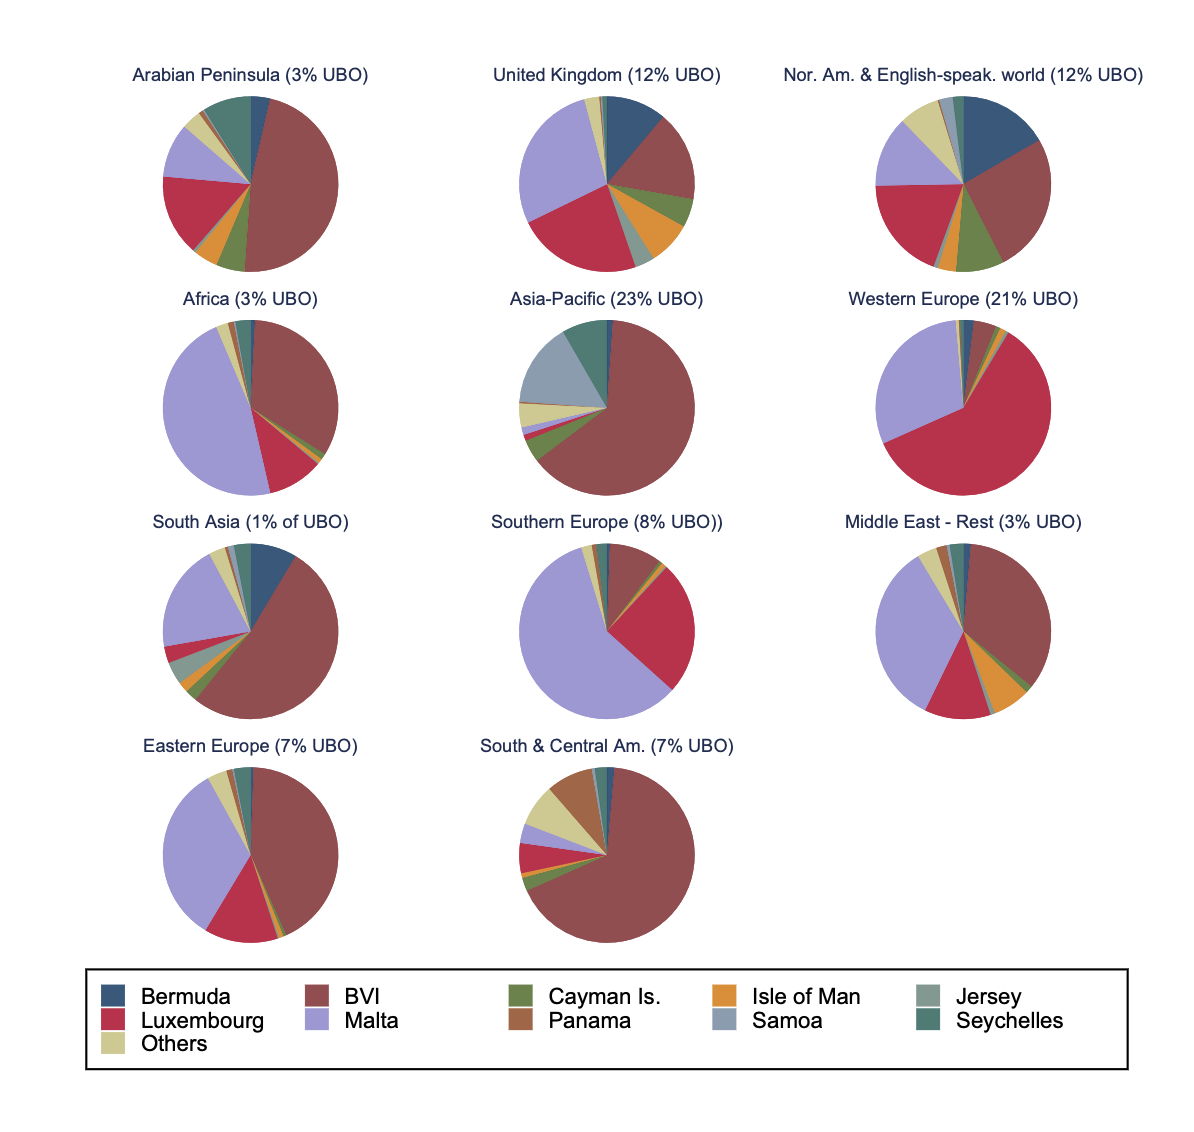
\includegraphics[width=1\textwidth]{Screenshot 2024-04-09 at 14.21.57.png}
    \caption{Frequent tax haven use by world region regarding ultimate beneficial ownership\protect\footnotemark}
    \label{fig:unique-label}
\end{figure}

\addtocounter{footnote}{0} % Adjust the counter if necessary
\footnotetext{This figure illustrates the most frequent tax havens used to incorporate overseas companies, defined by the region of the beneficial owner(s). It is put together by Bomare and Herry (2022), using restricted data on beneficial ownership and company data from the Bahamas Leaks, the Offshore Leaks, the Panama Papers, the Paradise Papers, OpenLux data, and CNBIOM data.  Source: (Bomare and Herry (2022)}

\begin{figure}[H]
    \centering
    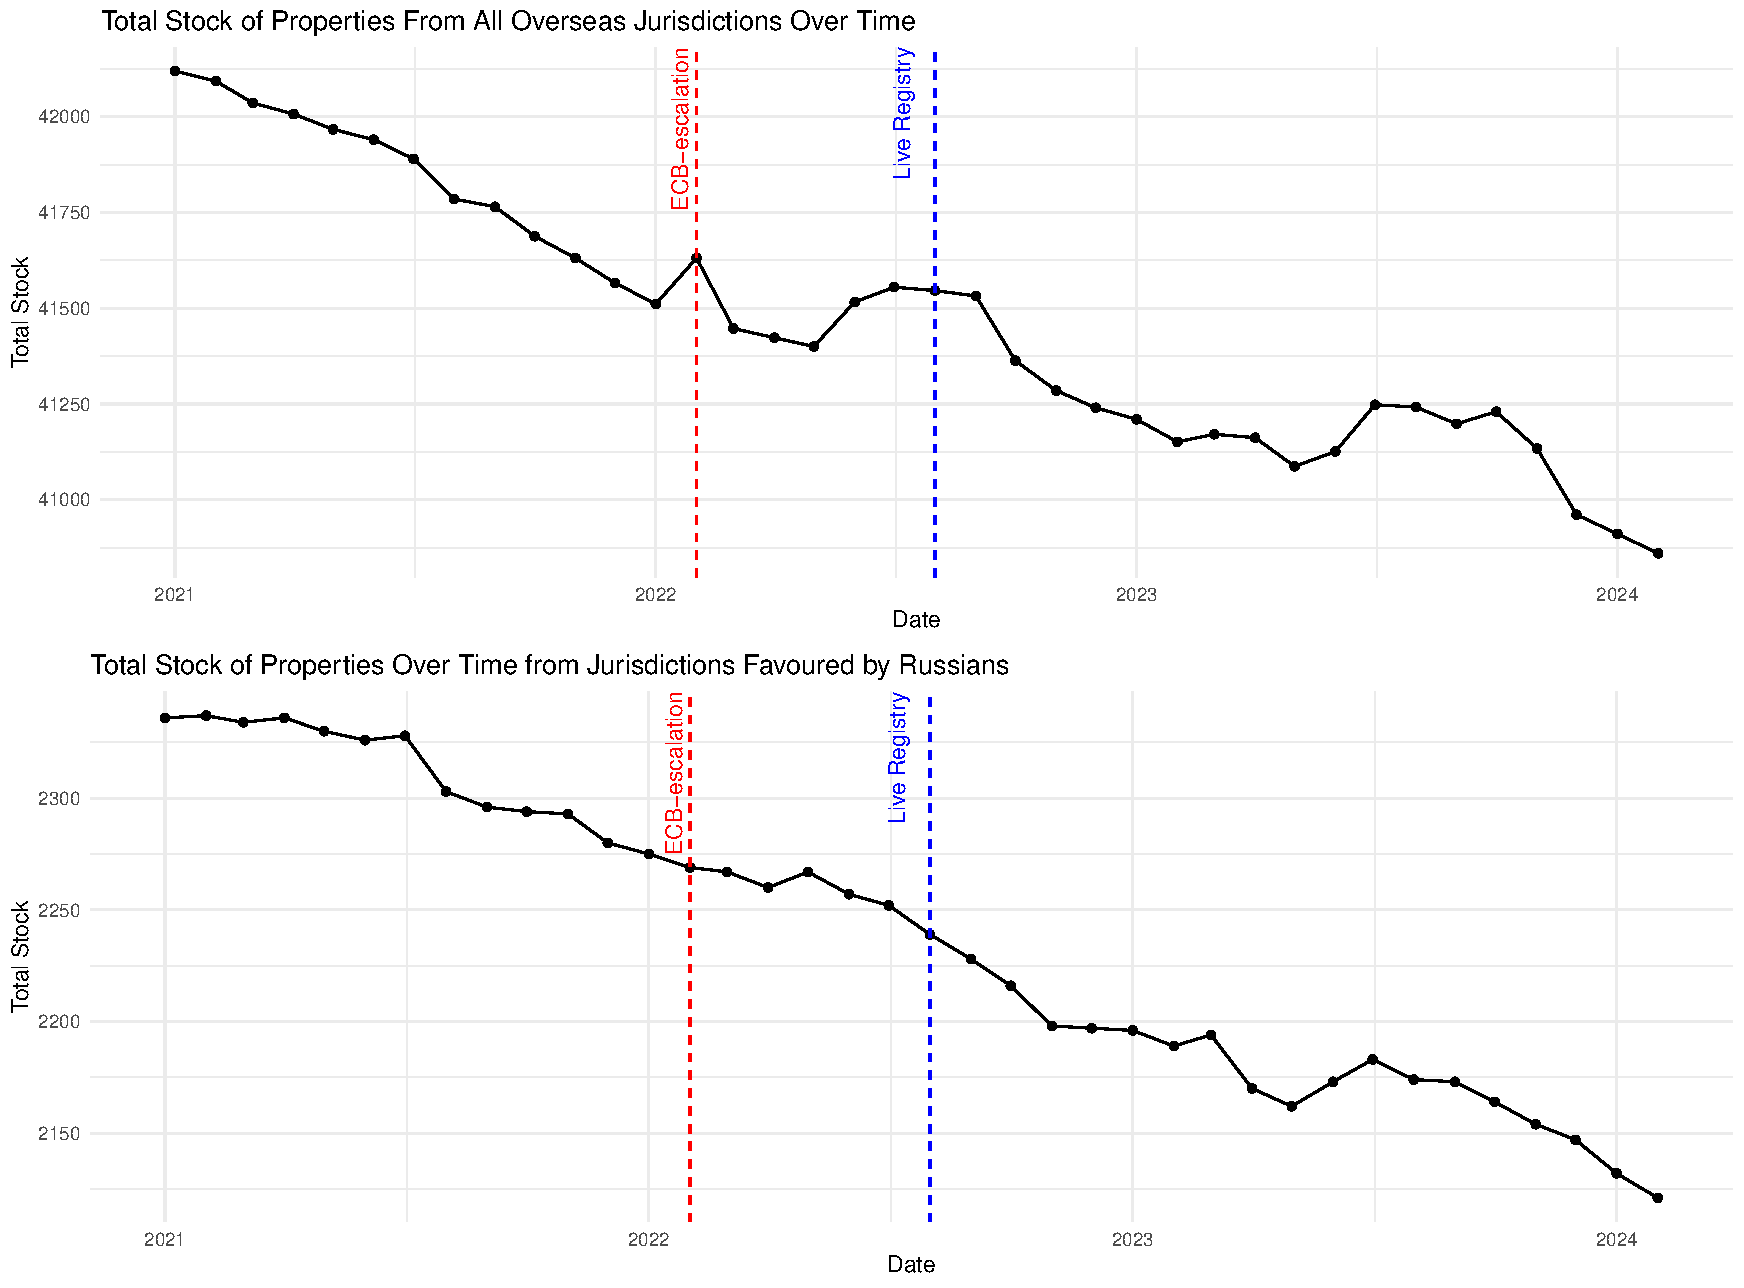
\includegraphics[width=\textwidth]{Rplot02.pdf}
    \caption{Total stock of property owned by all overseas companies and Russian favoured havens over time.\\ Source: (Author's Compilation)}
    \label{fig:enter-label}
\end{figure}

Figure 2 visualises several interesting trends in the data sample. Firstly, before the policy was introduced there was a negative trend in property ownership from all overseas jurisdictions and Russian favoured jurisdictions. When the ECB is introduced, as given by the dashed red line, the negative trend continues for Russian favoured havens, but this is no longer characterised by all other jurisdictions, as there is a positive trend in the stock of property ownership three months after the ECB was introduced. Crucially, this discrepancy in the trends could be evidence that transparency is adversely affecting Russian property investment, at least in the short run. The longer-run effects, after the registry goes live, we notice that the negative trends persist for both groups, which could be evidence of the limited longer-run implications of the transparency policy.
\newpage

\subsection{Classifying Districts Favoured by Russians}
To identify the properties held by Russians in certain London districts, I will use multiple sources. Firstly, research by Transparency International has found that since 2016, Russians linked to the Kremlin have purchased properties worth £1.5 billion. This includes £430 million in the City of Westminster, £230 million in Kensington and Chelsea, and £165 million in Camden. Other districts that have a high volume of properties associated with Russian illicit wealth are Lambeth, Brent, Southwark and Croydon (Transparency International UK 2022a). Therefore taking advantage of the concentration of wealth held within these identified districts will form the primary classification of districts used in the analysis.

In addition to this, I will also consider the agglomeration behaviour of certain nationalities identified by Bomare and Herry (2020). Figure 3 shows the concentration of properties purchased by companies registered in all overseas jurisdictions, from the OCOD data sample. Transactions of properties are concentrated in central districts. However, extending this relationship to Figure 4, the agglomerative behaviour becomes more distinct. Subfigure (f) displays the estimates of Russian property purchases characterised by the upper quintile of transactions. It is identified that most of these purchases take place in Enfield, Westminster, Kensington, Chelsea, and Richmond. Therefore, to obtain more robust results, I will include this alternative classification of districts in our estimates.


\begin{figure}[H]
    \centering
    \begin{subfigure}[b]{0.9\textwidth}
        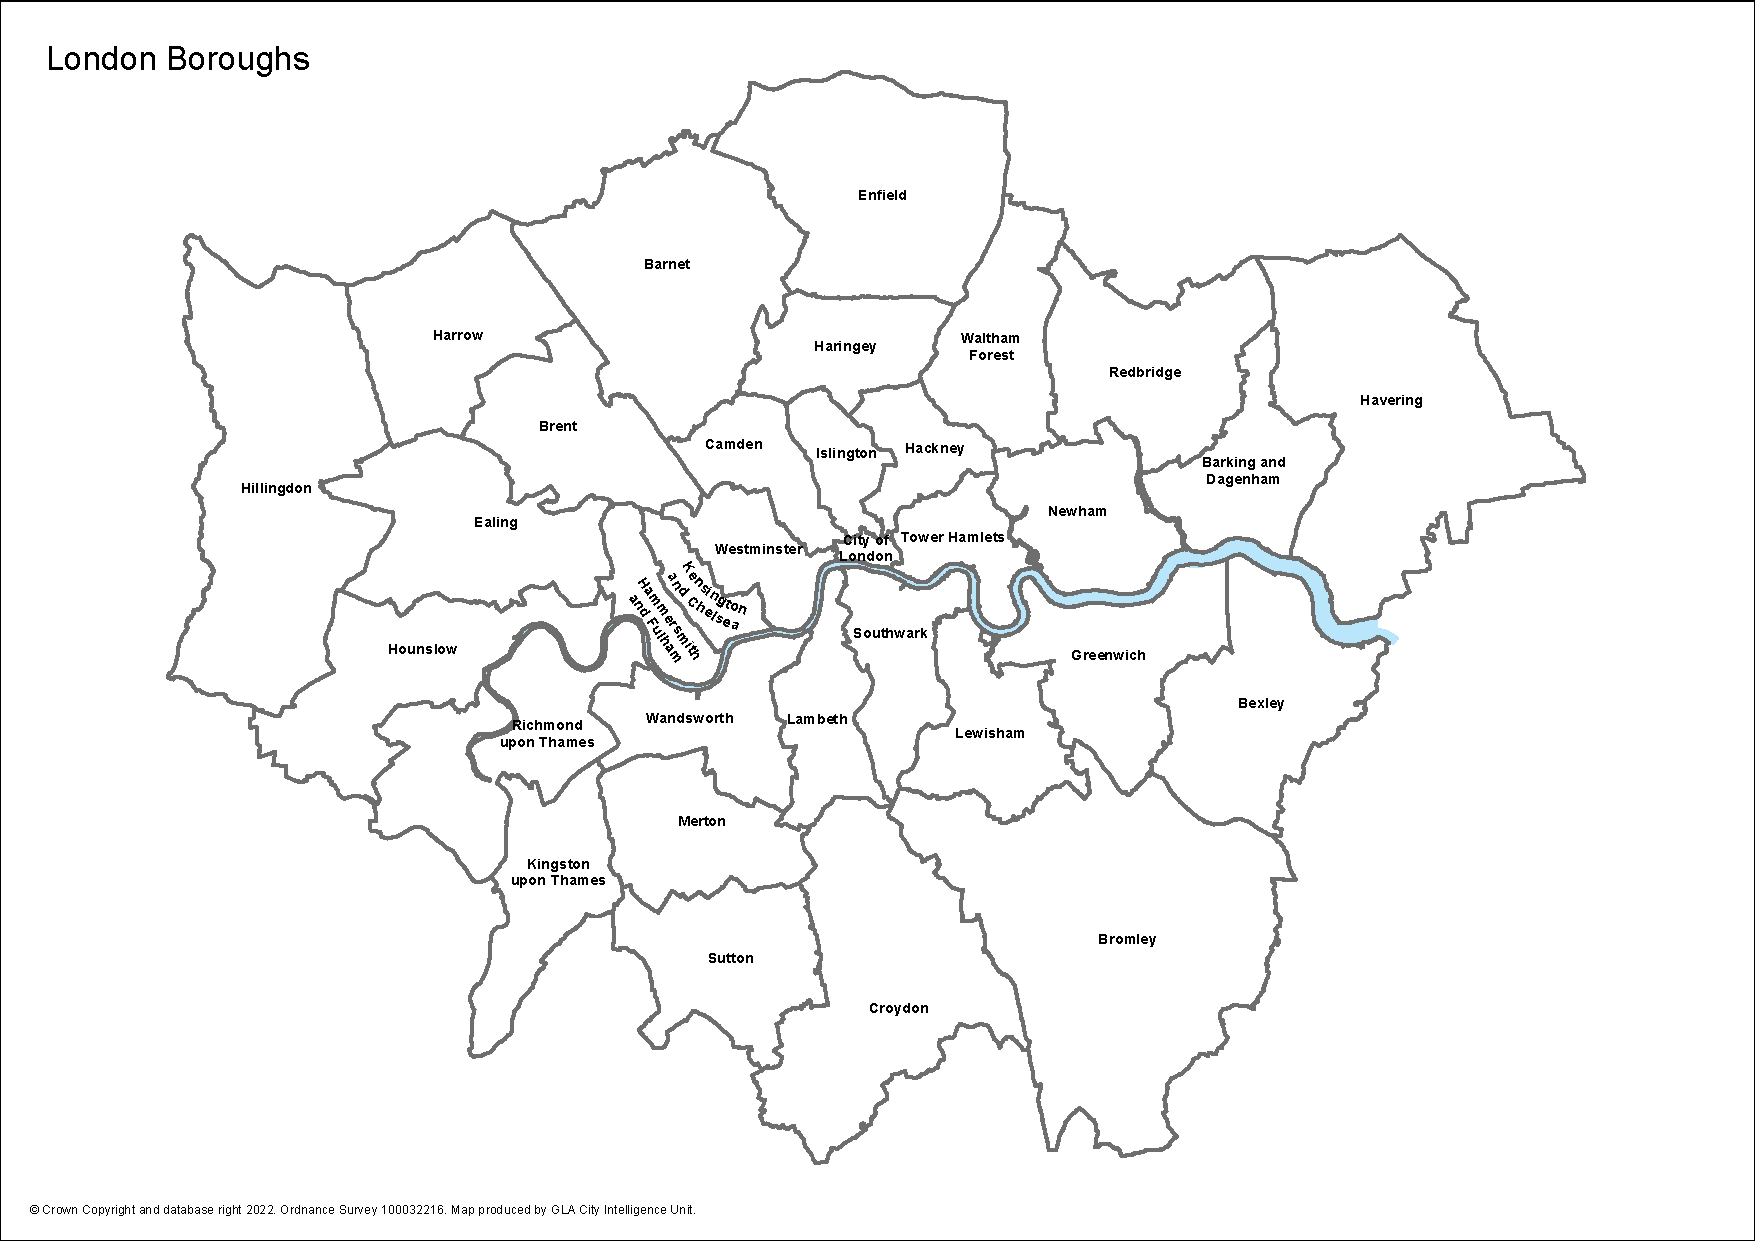
\includegraphics[width=\textwidth]{London_Borough_Boundary_Map_A4.pdf}
        \caption{Map of the districts in London}
        \label{fig:sub1}
    \end{subfigure}
    
    \begin{subfigure}[b]{0.9\textwidth}
        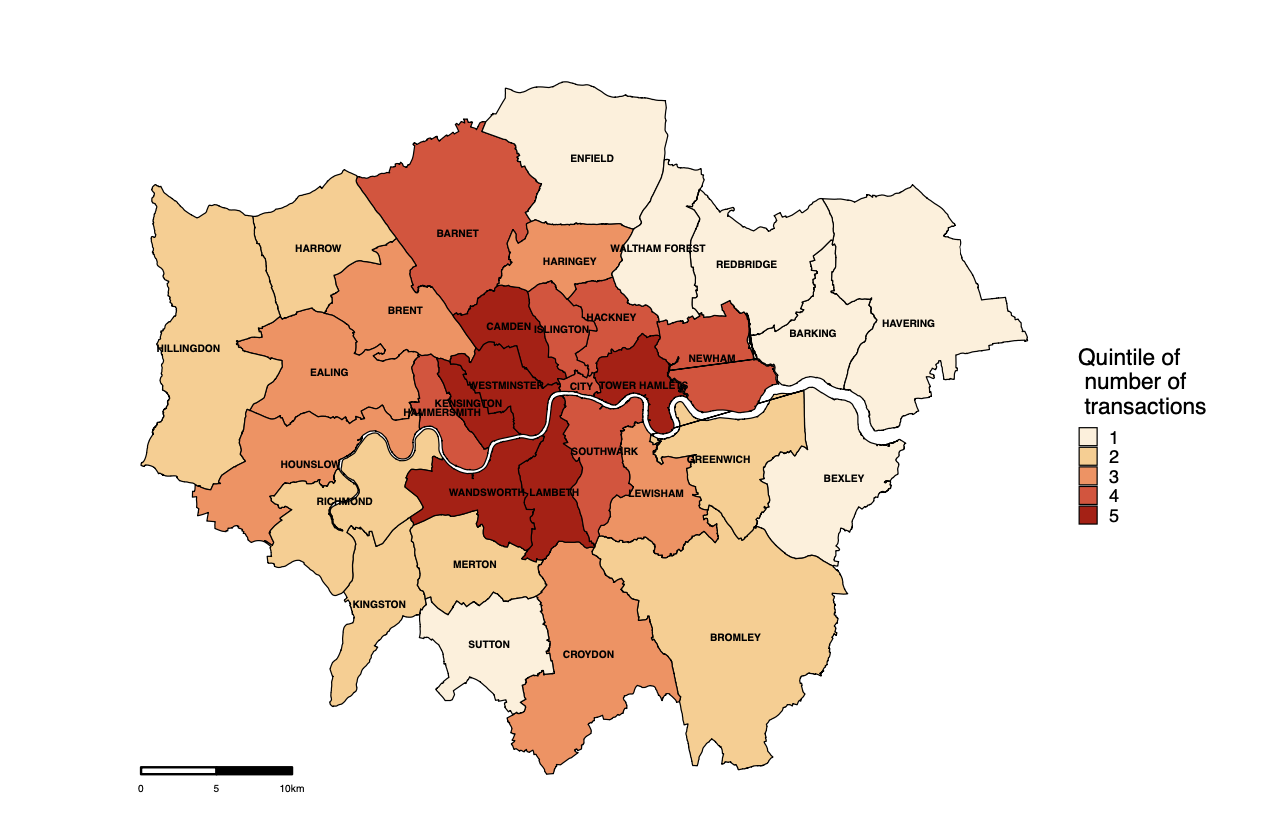
\includegraphics[width=\textwidth]{Screenshot 2024-04-09 at 10.27.40.png}
        \caption{Number of Overseas Purchases in London from the OCOD sample \footnotemark}
        \label{fig:sub2}
    \end{subfigure}
    \caption{Concentration of Overseas Property Ownership in London Districts }
\end{figure}

\footnotetext{This figure illustrates the locations of property purchases made by overseas firms in London from the OCOD data. The Greater London area is composed of 32 boroughs and the City of London. The boroughs are ranked in five quintiles based on the total number of purchases made by overseas firms over the period 2000-2020. Boroughs where overseas companies make the least purchases are denoted by quintile 1 and boroughs where these firms make the most purchases are denoted by quintile 5. Source: (Bomare and Herry (2022).}

\begin{figure}[H]
    \centering
    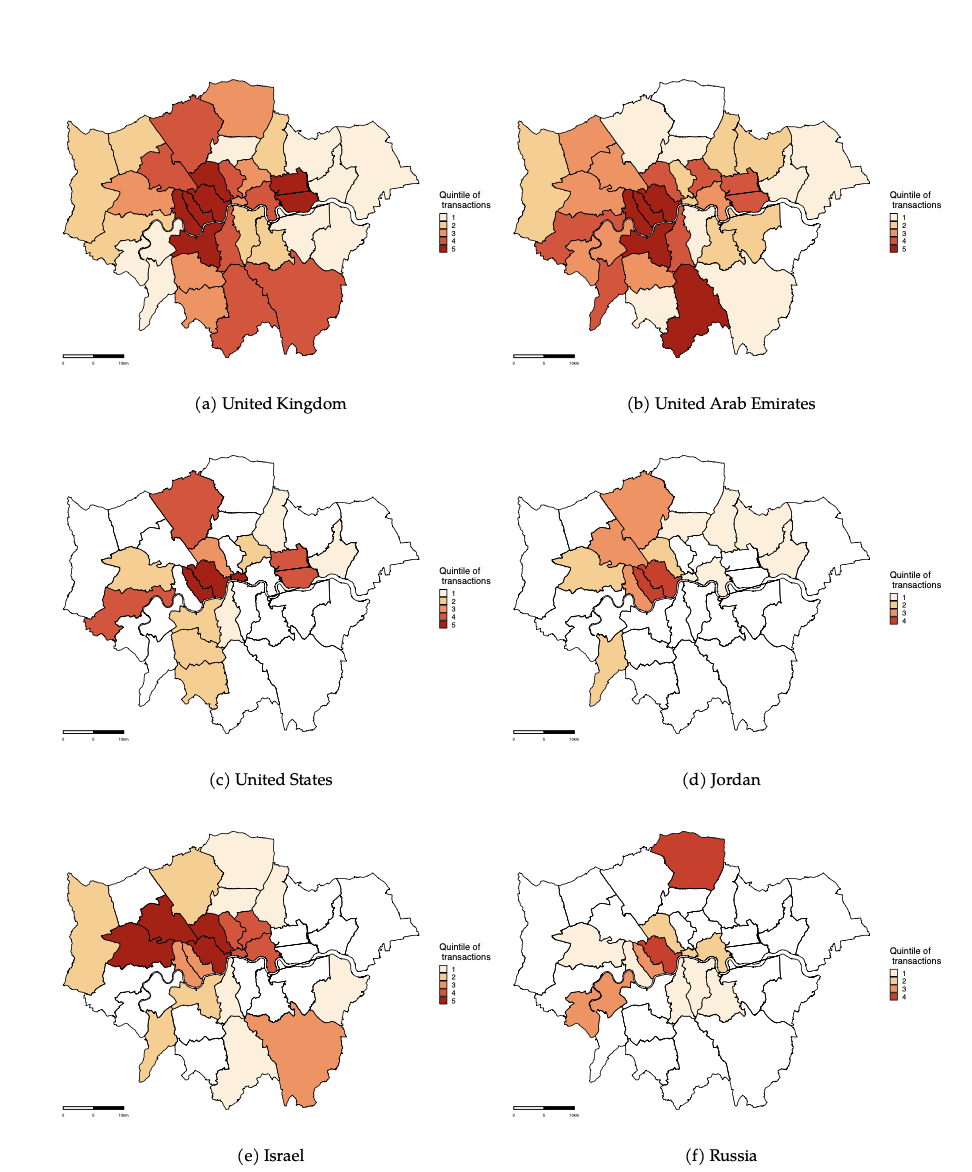
\includegraphics[width=\textwidth]{Screenshot 2024-04-09 at 09.58.02.png}
    \caption{District concentration of property purchases by identified buyers, by nationalities.\footnotemark}
    \label{fig:enter-label}
\end{figure}

\footnotetext{This figure illustrates the locations within London of purchases of property made by shell companies associated with various nationalities, as recorded by the OCOD. The boroughs are ranked in quintiles according to the total number of purchases from overseas companies from 1959-2020, this is the entire period covered by the OCOD. Source: (Bomare and Herry 2022).}


\begin{figure}[H]
    \centering
    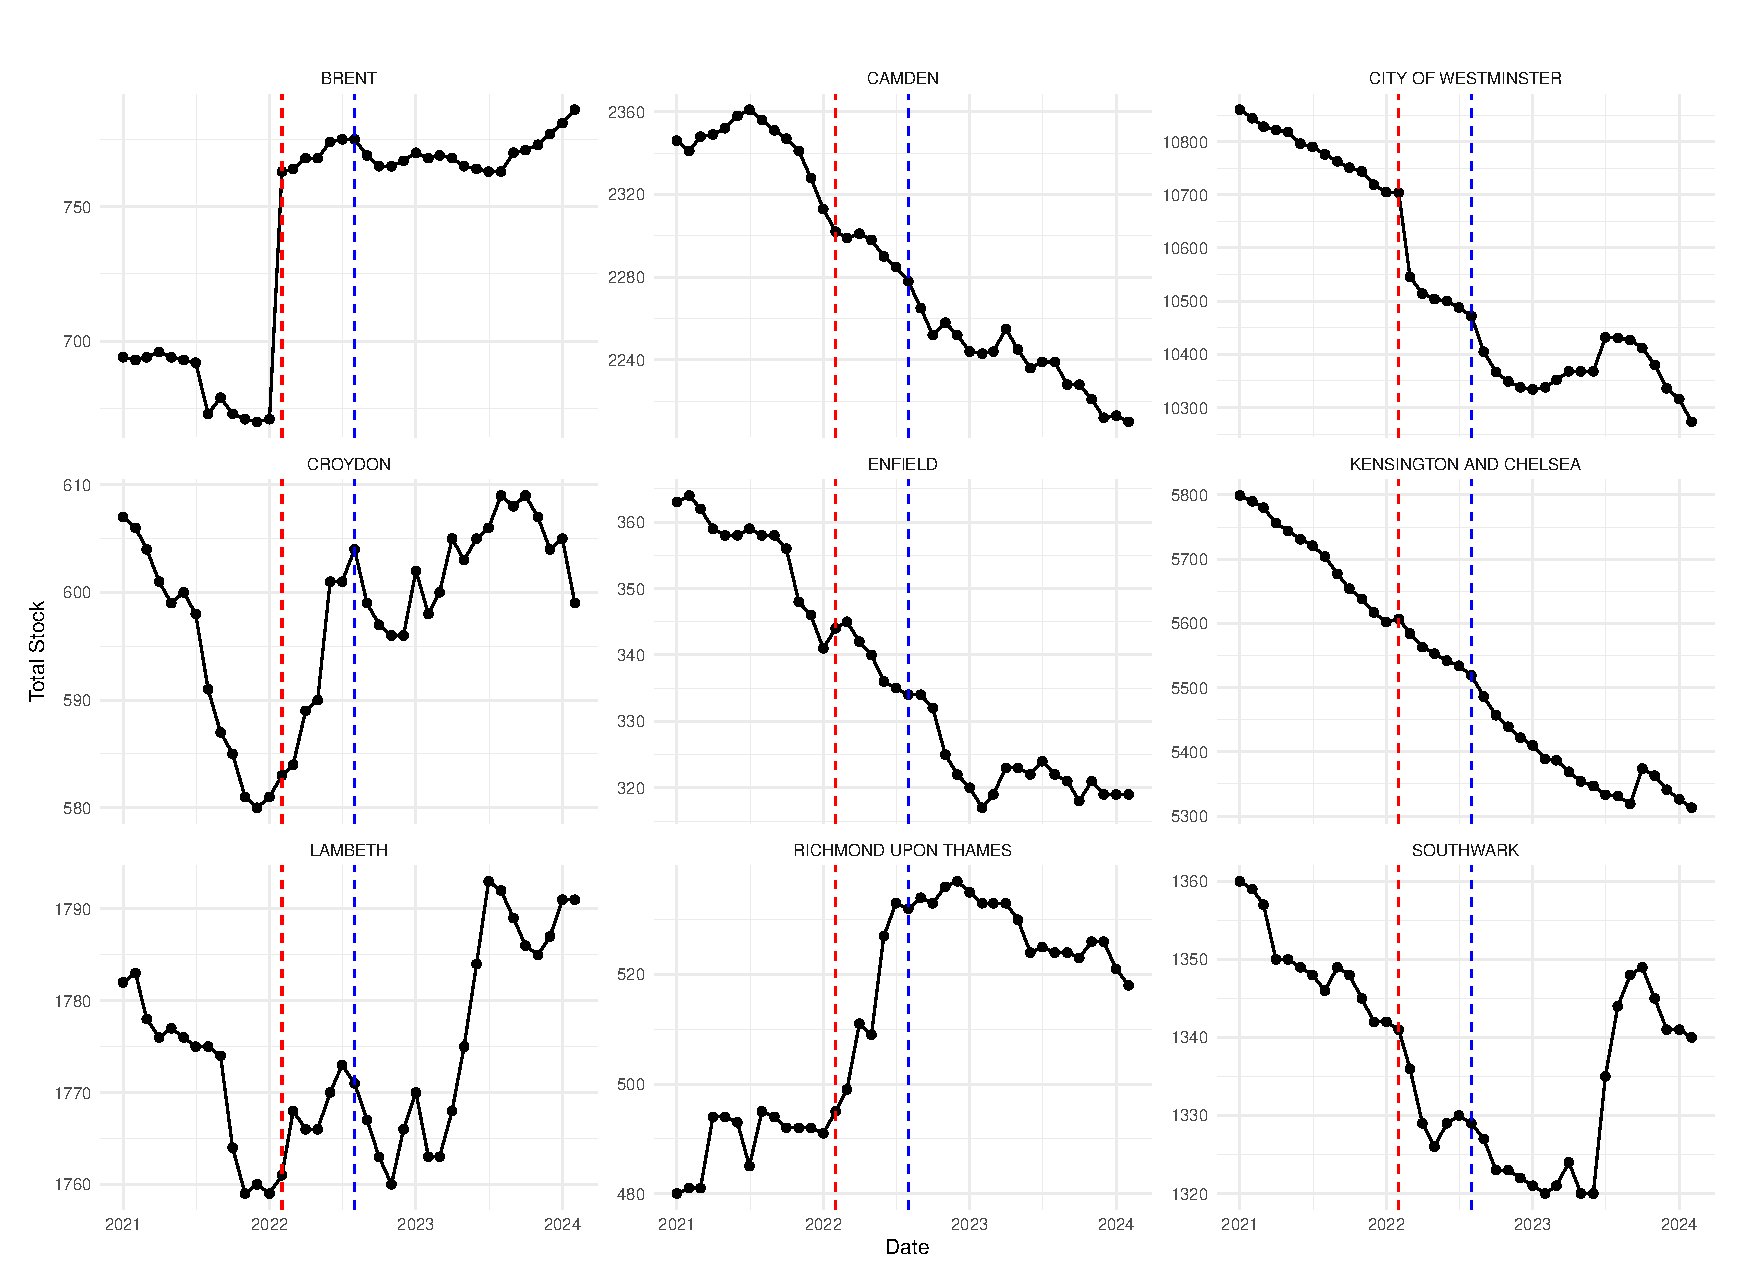
\includegraphics[width=\textwidth]{Rplot03.pdf}
    \caption{Total Stock of Property in Russian Identified Districts in London \\ Source: (Author's Compilation)}
    \label{fig:enter-label}
\end{figure}

Figure 5 shows the changes in the stock of property across various districts favoured by Russians. If we consider the districts that appear in both of our classifications, such as the City of Westminster and Kensington and Chelsea, we notice sharp declines in the stock of ownership in all these districts following the introduction of the ECB as shown by the dashed red line. This trend continues and becomes more apparent, particularly for Westminster, when the registry of beneficial ownership goes live (dashed blue line). However, some districts exhibit the opposite behaviour, and the stock of property ownership within these districts increases following the introduction of the ECB. For instance, Croydon and Lambeth show sharp increases initially, but once the registry goes live, there is then a negative trend. This could be evidence that individuals buy property in anticipation of the registry between the announcement of the ECB and when the registry goes live. Similarly, Brent and Richmond follow this same sharp increase following the ECB introduction, but they maintain a stable relationship before and after the registry goes live. Taken together, these trends in the data could suggest potential behavioural shifts by Russians from purchasing property within central to wider districts in light of attempts to introduce greater transparency.

\section{Empirical Framework}

\subsection{The Effect of the ECB Announcement on Offshore Investments in the London Property Market}

The main concern for this paper is to analyse the impact of the UK government's attempt to introduce greater transparency towards offshore property ownership made by Russians within the UK. Specifically, the impact following the fast-tracking of the Economic Crime Bill (ECB) and the establishment of the Overseas Registry following the Russian invasion of Ukraine. I proceed with my analysis, as mentioned, by using a series of difference-in-difference estimations. With havens favoured by Russian nationals as my primary treatment group and all other overseas jurisdictions as the control group. The baseline regression is the following:
\begin{equation}
S_{it} = \beta \times Rus_i \times Post_t + \gamma_i + \theta_t + \epsilon_{it}
\end{equation}

Where $S_{it}$ denotes the stock or the purchase/sale of properties owned by companies registered in jurisdiction $i$ within a particular month $t$. The variable $Rus_i$ is a binary dummy variable equal to one if the jurisdiction is considered to be favoured by Russians and $Post_t$ is an indicator variable equal to one on and after February 2022 (escalation of the ECB). The parameters $\gamma_i$ and $\theta_t$ capture jurisdiction and monthly fixed effects respectively, and the standard erros $\epsilon_{it}$ are clustered at the jurisdiction level. Crucially, the difference in difference coefficient $\beta$ estimates the difference in investment made by companies based in havens favoured by Russians and every other overseas jurisdiction. 

\paragraph{Event Study}To examine the changes in the purchases and sales by Russians over time following the introduction of the ECB, I will also estimate the event study using the specifications from the baseline regression: 
\begin{equation}
P_{it} = \sum^{-1}_{\tau=-14}\beta_\tau({Rus_{i}\times{Post_{\tau,t}})}+\sum^{24}_{\tau=0}\beta_\tau({Rus_{i}}\times{Post_{\tau,t})} + \gamma_i + \theta_t + \epsilon_{it}
\end{equation}

From equation (3), $P_{it}$ is the stock, purchase/sale of property owned by companies in jurisdiction $i$ at month $t$. In this model I have included the summation of interaction terms between our Russian indicator variable and a series of time dummies around the introduction of the ECB. Specifically, $Rus_i$ takes the same values as before, but $Post_{\tau,t}$ are a set of time dummies that correspond to monthly periods relative to the ECB re-tabling. Here, $\beta_\tau$ captures the differences in investment made by companies based in havens favoured by Russians and every other jurisdiction in each of the monthly periods $\tau$.  

\paragraph{Other treatment groups} I will also extend the analysis to include other treatment groups to capture a wider effect of transparency within the London offshore property market. By extending the baseline regression, but now but including the use of havens favoured by different groups classified above. Specifically, estimated by the following equations: 


\begin{itemize}
\item All jurisdictions considered havens as defined by (Menkhoff and Miethe 2019): 
\begin{equation}
S_{it} = \beta \times Haven_i \times Post_t + \gamma_i + \theta_t + \epsilon_{it}
\end{equation}

\item Havens used by the upper quartile of highly corrupt countries as identified by Transparency International:
\begin{equation}
S_{it} = \beta \times CPI_i \times Post_t + \gamma_i + \theta_t + \epsilon_{it}
\end{equation}
\item Havens used by countries that are signatories to the Automatic Exchange of Information (AEOI) as identified by (Bomare and Herry 2022):
\begin{equation}
S_{it} = \beta \times AEOI_i \times Post_t + \gamma_i + \theta_t + \epsilon_{it}
\end{equation}
\end{itemize}

I will also consider the event study for each respective treatment group, denoted by $(treat_i)$. Given by the general specification: 

\begin{equation}
P_{it} = \sum^{-1}_{\tau=-14}\beta_\tau({treat_{i}\times{Post_{\tau,t}})}+\sum^{24}_{\tau=0}\beta_\tau({treat_{i}}\times{Post_{\tau,t})} + \gamma_i + \theta_t + \epsilon_{it}
\end{equation}

\subsection{Measuring the Effect of the ECB on District Level Foreign Investment}

It was found that there was minimal correlation between jurisdictions favoured by Russians and other treatment groups. There still exists the problem that some havens favoured by Russians could still be used by other groups not included in our estimation. Therefore, to deepen the classification of Russian beneficial owners, I use a triple difference in difference estimation that interacts with districts within London that are notoriously known to hide Russian wealth. The estimation is based on the following specifications: 

\begin{equation}
S_{itj} = \eta (Rus_{itj} \times Post_{itj}\times{Dist_{itj}}) + \gamma_{i} + \theta_{t} + \delta_{j} + \epsilon_{itj}
\end{equation}

In this specification, I include the same controls from equation (1) but now interact the dummy variable $Dist_{itj}$, with the treatment event and also the Russian haven dummy. $Dist_{itj}$ also equals one if the district is identified to be commonly associated with illicit Russian financial activities. The parameters $\gamma_{i}$, $\theta_{t}$ and $\delta_{j}$ capture jurisdiction, monthly and district fixed effects respectively. The coefficient $\eta$ estimates the difference in investments between companies registered in havens preferred by Russians, who own property in Russian-favoured London districts, and companies that are registered in non-Russian-favoured jurisdictions that own properties outside the Russian-favoured districts. 


\paragraph{Event Study} I also estimate the event study version of equation (8) that takes the same explanation as equation (3), but I have also included the additional $Dist_{itj}$ interaction term:
\begin{equation}
P_{itj} =\sum^{-1}_{\tau=-14}\eta_\tau({Rus_{itj}}\times Post_{\tau,itj}\times{Dist_{itj})}+\sum^{24}_{\tau=0}\eta_\tau({Rus_{itj}}\times Post_{\tau,itj}\times{Dist_{itj})} + \gamma_i + \theta_{t} + \delta_{j} + \epsilon_{itj}
\end{equation}


\section{Results}
\subsection{Investment changes by Russian nationals}
Table 1 presents the results from our baseline regression estimation. In addition to estimating the effect in the number of properties, I also include the inverse hyperbolic sine transformation for each of our dependent variables. A justification for this is that our sample dataset contains many zero values which in this case is significant for our estimates as it captures marginal changes in transactional behaviour. There are also in some cases many negative value data points that cannot be directly applied to the logarithmic transformation. Because the log transformation can only be applied to strictly positive variables, there have been several studies that add an arbitrarily small positive number to variables with zero values or replace zero values with an arbitrarily small positive number before applying the log transformation. However, these arbitrary manipulations of the variables change the original structure of the data (Duan et al., 1983), such that this arbitrary replacement can substantially affect the empirical results (N’guesan et al., 2017). Crucially, the inverse hyperbolic transformation (ihs) can be used as an alternative to the log transformation. Because it can be applied to negative and zero values without any arbitrary manipulations on the variables of interest. It has also been argued that the transformation allows for a similar interpretation of the regression results following a log transformation (see, Carroll et al., 2003; Carboni, 2012; Ravallion, 2017; Bellemare and Wichman, 2020). 

What our results show is that following the Russian invasion of Ukraine and the subsequent re-escalation of the ECB, there is a notable statistically significant fall in the total number of properties owned by offshore companies that are incorporated in havens favoured by Russians, however, this relationship does not hold or remain statistically significant when the IHS transformation is applied. To observe specific transactional behaviour, I extend the analysis that focuses on the purchase and sales of properties. We find that following the policy implementation there is a statistically significant positive effect on both. Where the purchases of properties increased by approximately 9.64${\%}$ and the sales are predicted to increase by around 20${\%}$ following the policies’ introduction. Also included in our estimates is the effect the ECB has had on the aggregate value of properties, however, there is no statistical significance.

To address potential endogeneity problems, where some of the havens favoured by Russians are also used by other high-risk groups. I include an additional layer of focus by using the agglomeration behaviour of Russian nationals within certain London districts. By modelling a triple difference in difference approach, we find the results to be more aligned with our expected estimations. The stock of properties within Russian-favoured districts owned by companies registered in Russian-favoured havens remains negative following the introduction of the ECB, but no longer remains statistically significant. However, interestingly, we find that the purchases of properties within these certain districts fall and are marginally negative, however, the inverse hyperbolic transformation of purchases remains positive and predicts a 2.4${\%}$ increase in purchases following the policy introduction.  Equally, the sale of properties remains positive, but the effect is relatively marginal concerning the previous specification and the ihs transformation is no longer statistically significant. However, there is evidence to show that the aggregate volume of sales in terms of value has increased by approximately 26${\%}$ within these specific districts. 

To improve the validity of our estimates and address the concern that there are havens used by different high-risk groups. I also re-specified the models by limiting the threshold of havens and districts used by Russians based on the percentage of beneficial ownership, specifically to the upper quartile of havens in the Russian column given in Figure (1). I also extend this to the triple difference in difference model, using the same classification of havens used by Russians, as mentioned, but now I use the districts identified by Bomare and Herry (2022), as mentioned, specifically to Enfield, Richmond, Westminster, Kensington, and Chelsea. These districts have the highest concentration of property ownership by Russians as identified in the OCOD dataset. Limiting the havens and districts that are increasingly favoured by Russians, helps reduce some of the multicollinearity between havens and districts used by other groups. The results are shown in the appendix. 

\begin{table}[H]
\caption{Difference-in-difference and Triple Difference-in-difference estimation of transactions from Jurisdictions favoured by Russians}
\label{yourLabelHere}
\centering
  \begin{adjustbox}{width=1.25\textwidth,center}
  \begin{threeparttable}
\begin{tabular}{@{}lccccccccc@{}}
\toprule
 & \multicolumn{3}{c}{Stock} & \multicolumn{3}{c}{Purchase} & \multicolumn{3}{c}{Sale} \\
\cmidrule(lr){2-4} \cmidrule(lr){5-7} \cmidrule(lr){8-10}
& Stock & ihs(Stock) & ihs(£Volume) & Purchase & ihs(Purchase) & ihs(£Volume) & Sale & ihs(Sale) & ihs(£Volume) \\
\midrule
(i) Russia $\times$ Post & $-$44.767$^{***}$ & 0.0002 & -0.049 & 1.884$^{***}$ & 0.096$^{*}$ & -0.021 & 2.105$^{***}$ & 0.203$^{***}$ & 0.542 \\
& (3.464) & (0.015) &  (0.086) & (0.411) & (0.045) & (0.457) & (0.321) & (0.049) & (0.430) \\
\midrule
Observations & 6,779 & 6,779 & 6,779 & 6,591 & 6,591 & 6,591 & 6,591 & 6,591 & 6,591 \\
\toprule
(ii) Russia$\times$Post$\times$District & $-$9.072 & 0.008 & 0.051 & -0.113$^{**}$ & 0.024$^{**}$ & 0.014 & 0.090$^{*}$ & 0.004 & 0.257$^{*}$ \\
& (6.565) & (0.047) & (0.087) & (0.056) & (0.012) & (0.149) & (0.047) & (0.014) & (0.142)\\
\midrule
Observations & 56,665 & 56,665 & 56,665 & 56,665 & 56,665 & 56,665 & 56,665 & 56,665 & 56,665 \\
\bottomrule
\end{tabular}
\begin{tablenotes}
\item
    Note: This table presents the difference-in-difference estimates and the triple difference-in-difference estimates of the total stock, purchase and sale of London property by offshore companies situated in overseas jurisdictions favoured by Russians. Also included are the inverse hyperbolic sine transformation of each of the dependent variables respectively. (i) The treatment group are havens favoured by Russians and all other overseas jurisdictions as the control groups. (ii) The treatment groups are havens favoured by Russians and London districts favoured by Russians, and all other overseas jurisdictions and London districts acting as the control. Standard errors are clustered at the overseas jurisdiction level. $^{*}$p$<$0.1; $^{**}$p$<$0.05; $^{***}$p$<$0.01
\end{tablenotes}
\end{threeparttable}
\end{adjustbox}
\end{table}


\paragraph{Event Study}  Figure (7) shows the event study estimations of equations (3) and (8). The event study allows us to observe the investment behaviour and transactions made by Russian nationals around the treatment period given by the dashed vertical line, at a time to treat value zero. These two figures show us the coefficient estimates of the inverse hyperbolic sign on property purchases/sales with 14 monthly leads before the treatment period and lags of 24 months. Focusing first on the property purchases from the baseline difference in difference (DiD) specification given in Figure (7a), we observe highly fluctuating patterns. Before the Russian invasion and the re-tabling of the ECB, we noticed a negative trend in the coefficient estimates that appeared to increase a month before the treatment period. There is then an immediate drop after the policy is introduced that is followed by an upward trend up to when the registry goes live, as indicated by the dashed blue line, after the registry is introduced, there are subsequent fluctuations following the treatment period. In contrast, when we incorporate specific district characteristics into our model, as represented by (DDD), the coefficient estimates are smaller in magnitude but are increasingly statistically significant. The pattern also deviates from the original estimates in that there are marginal variations before the policy introduction. There appears to be a lagged effect in that we notice a negative trend in the coefficient estimates four months after the policy was introduced that is short-lived as there is greater variation seven months after the treatment period.  

When we extend our analysis to Figure (7b), there exists a consistent relationship between our two estimates of property sales. From our broader estimates on classifying Russian nationals by their use of havens, the baseline difference in difference specification (DiD) suggests that there exists a positive relationship in property sales before and after the re-tabling of the ECB, due to the large confidence intervals around the coefficient estimates it is difficult to give any causal interpretation. However, after classifying Russian nationals by their use of specific havens and districts in London our estimates from the triple difference in difference (DDD) specification, on property sales, remain positive and are increasingly statistically significant. There is more of a revealing pattern in that we observe a marginal positive trend in property sales before the treatment period that is followed by relatively larger variations after that, there is also evidence similar to the purchase of property in that there is a lagged effect, specifically a month after the registry goes live, we observe a peak in property sales that is then followed by relatively marginal cyclical variations.


\begin{figure}[H]
    \centering
    \begin{subfigure}[b]{0.9\textwidth}
    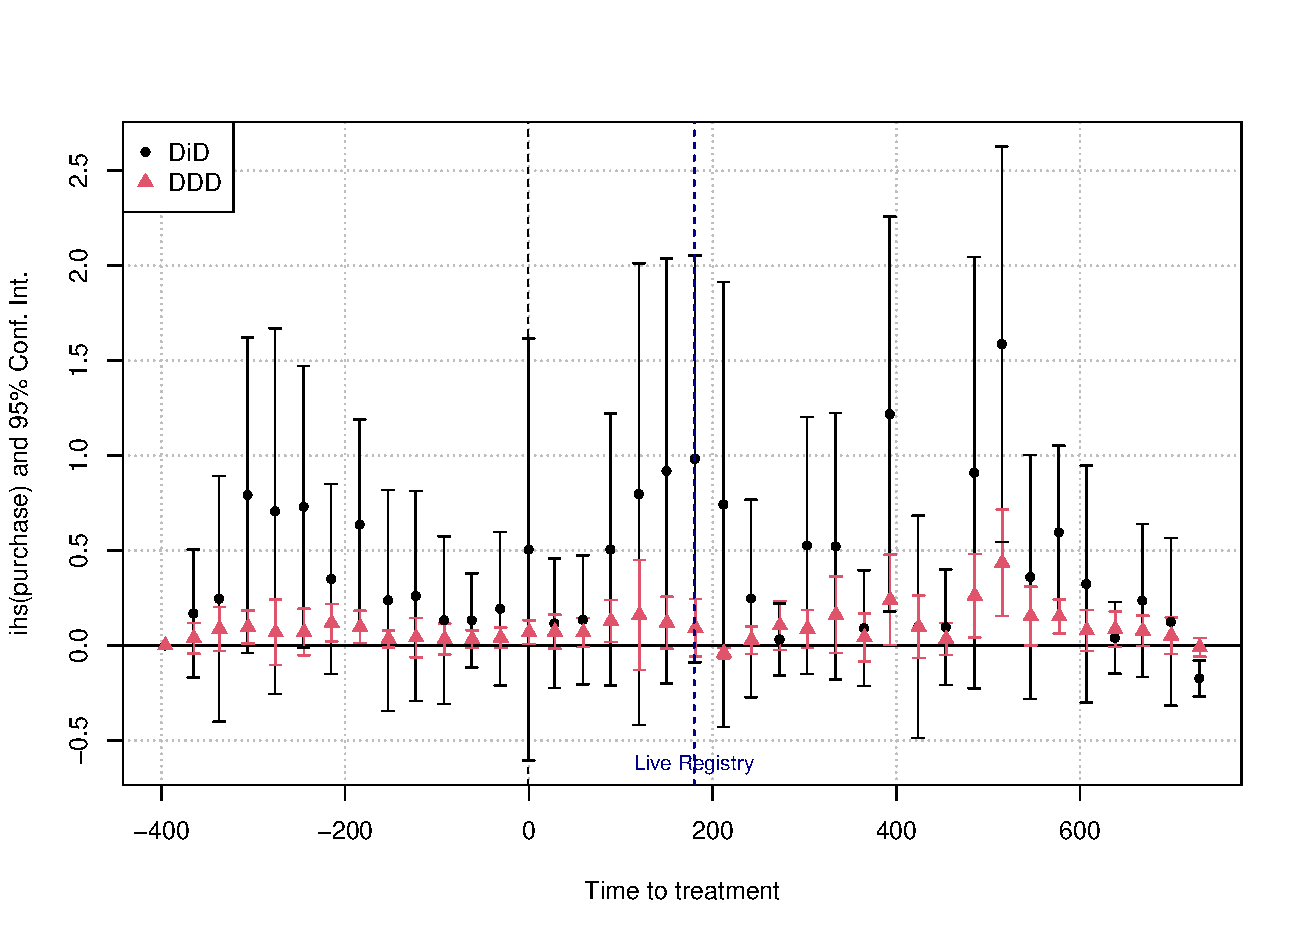
\includegraphics[width=1\linewidth]{ihs(Purchase)_Russia_Count.pdf}        
    \caption{Difference-in-difference (DiD) and Triple difference-in-difference (DDD) specification coefficient estimates on monthly property purchases from Russian favoured overseas jurisdictions.}
        \label{fig:purchase}
    \end{subfigure}
    
    \begin{subfigure}[b]{0.9\textwidth}
    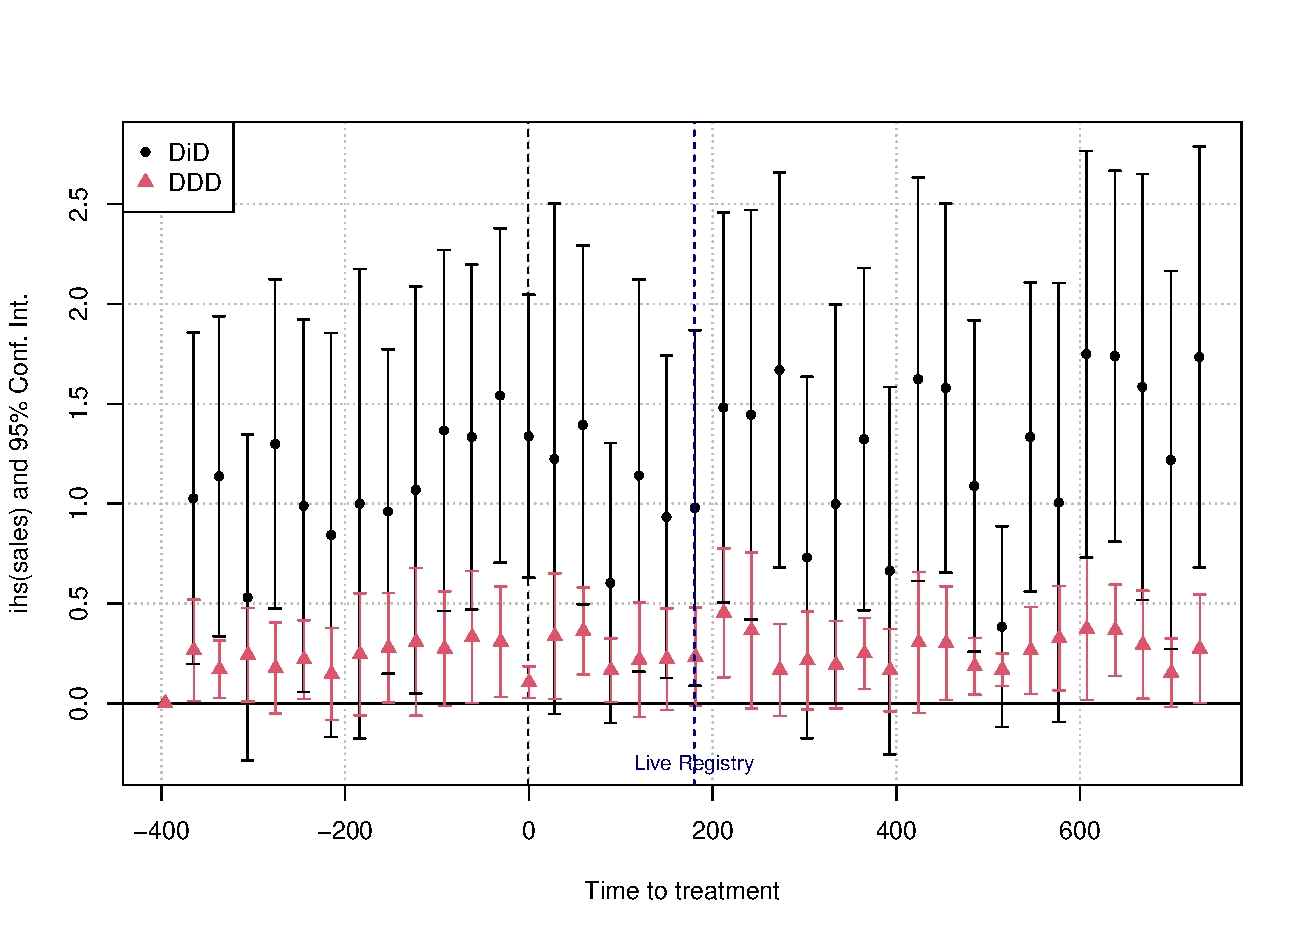
\includegraphics[width=1\linewidth]{ihs(Sale)_Russia_Count.pdf}
        \caption{Difference-in-difference (DiD) and Triple difference-in-difference (DDD) specification coefficient estimates on monthly property sales from Russian favoured overseas jurisdictions.}
        \label{fig:sale}
    \end{subfigure}
    \caption{Event study coefficient estimates on the inverse hyperbolic sine transformation of monthly property purchases and sales made by companies registered in Russian favoured tax havens. Source: (Author's Compilation).}
    \label{fig:overall}
\end{figure}



\subsection{Investment changes through havens favoured by different treatment groups}
To examine the broader impact of increased transparency on the offshore property market, I extend the analysis to include additional treatment groups. The results of the baseline difference in difference are presented in Table 3. When comparing all overseas jurisdictions considered havens against non-havens, there is a statistically significant decrease in the stock of property ownership. This trend is also observed in highly corrupt countries. However, the results from countries that are signatories to the Common Reporting Standard (CRS) show a completely different relationship. The introduction of the Economic Crime Bill (ECB) has not deterred the total stock of ownership. This could indicate that these countries have a greater incentive to conceal their beneficial ownership and avoid complying with the registry, in light of their commitment to the CRS.

When it comes to the purchase of properties, the results are not entirely clear. It appears that purchases made by all tax havens show no significance, and there is some evidence to suggest an 8.9{\%} decrease in purchases made by highly corrupt countries. However, what remains consistent is that there is a statistically significant positive relationship in the purchases made by countries participating in the Automatic Exchange of Information (AEOI) scheme. This positive relationship is seen not only in the number of properties purchased but also in the overall value of these purchases, which is estimated to have increased by 75${\%}$. In contrast, there is a statistically significant increase in property sales across all groups. All havens show an increase of approximately 14.9${\%}$ in the number of property sales, with a 42.5${\%}$ increase in the aggregate sale value. Additionally, there is an estimated increase in the number of property sales made by CPI and AEOI countries of 19.7${\%}$ and 31.6${\%}$, respectively.


\begin{table}[H]
\caption{Difference-in-difference estimates of  transactions from Jurisdictions favoured by different treatment groups}
\label{yourLabelHere}
\centering
\large % Adjust font size as needed
  \begin{adjustbox}{width=1.25\textwidth,center}
\begin{threeparttable}
\begin{tabular}{@{}lccccccccc@{}}
\toprule
 & \multicolumn{3}{c}{Stock} & \multicolumn{3}{c}{Purchase} & \multicolumn{3}{c}{Sale} \\
\cmidrule{2-4} \cmidrule{5-7} \cmidrule{8-10}
& Stock & ihs(Stock) & ihs(£Volume) & Purchase & ihs(Purchase) & ihs(£Volume) & Sale & ihs(Sale) & ihs(£Volume) \\
\midrule
(i) All havens$\times$POST & $-$13.511$^{***}$ & 0.009 & $-$0.052 & 0.338 & 0.019 & 0.090 & 0.764$^{***}$ & 0.149$^{***}$ & 0.425$^{*}$ \\
& (1.811) & (0.008) &  (0.045) & (0.221) & (0.023) & (0.082) & (0.166) & (0.025) & (0.409) \\
\midrule
(ii) CPI$\times$POST & $-$7.008$^{**}$ & $-$0.014 & $-$0.037 & $-$0.263 & $-$0.089$^{**}$ & 0.639 & 0.560$^{*}$ & 0.197$^{***}$ & 0.223 \\
 & (3.337) & (0.014) & (0.082) & (0.391) & (0.045) & (0.435) & (0.305) & (0.047) & (0.142)\\
\midrule
(iii) AEOI-signatories$\times$POST & 24.921$^{***}$& $-$0.016 & $-$0.046 & 1.296$^{***}$ & $-$0.033 & 0.749$^{*}$ & 2.095$^{***}$ & 0.316$^{***}$ & 0.096 \\ 
& (3.324) & (0.014) & (0.082) & (0.391) & (0.045)  & (0.435) & (0.305) & (0.047) & (0.409) \\ 
\midrule
Observations & 56,665 & 56,665 & 56,665 & 56,665 & 56,665 & 56,665 & 56,665 & 56,665 & 56,665 \\
\bottomrule
\end{tabular}
\begin{tablenotes}
    \item Note: This table presents the difference-in-difference estimates of the total stock, purchase and sale of London property by offshore companies situated in overseas jurisdictions as previously defined. The measurement for analysis is an overseas jurisdiction, with a treatment period of February 2022 (The Month of the Russian invasion of Ukraine and the re-tabling of the ECB). (i) The treatment group are all havens classified by Menkhoff and Miethe 2019, and all other jurisdictions act as the control group. (ii) The treatment group are countries that fall in the bottom quartile of Transparency International's Corruption Perceptions Index. (iii) The havens that are most favoured by countries that are from CRS/AEOI participating countries. Standard errors are clustered at the overseas jurisdiction level.    $^{*}$p$<$0.1; $^{**}$p$<$0.05; $^{***}$p$<$0.01
\end{tablenotes}
\end{threeparttable}
\end{adjustbox}
\end{table}

\begin{figure}[H]
    \centering
    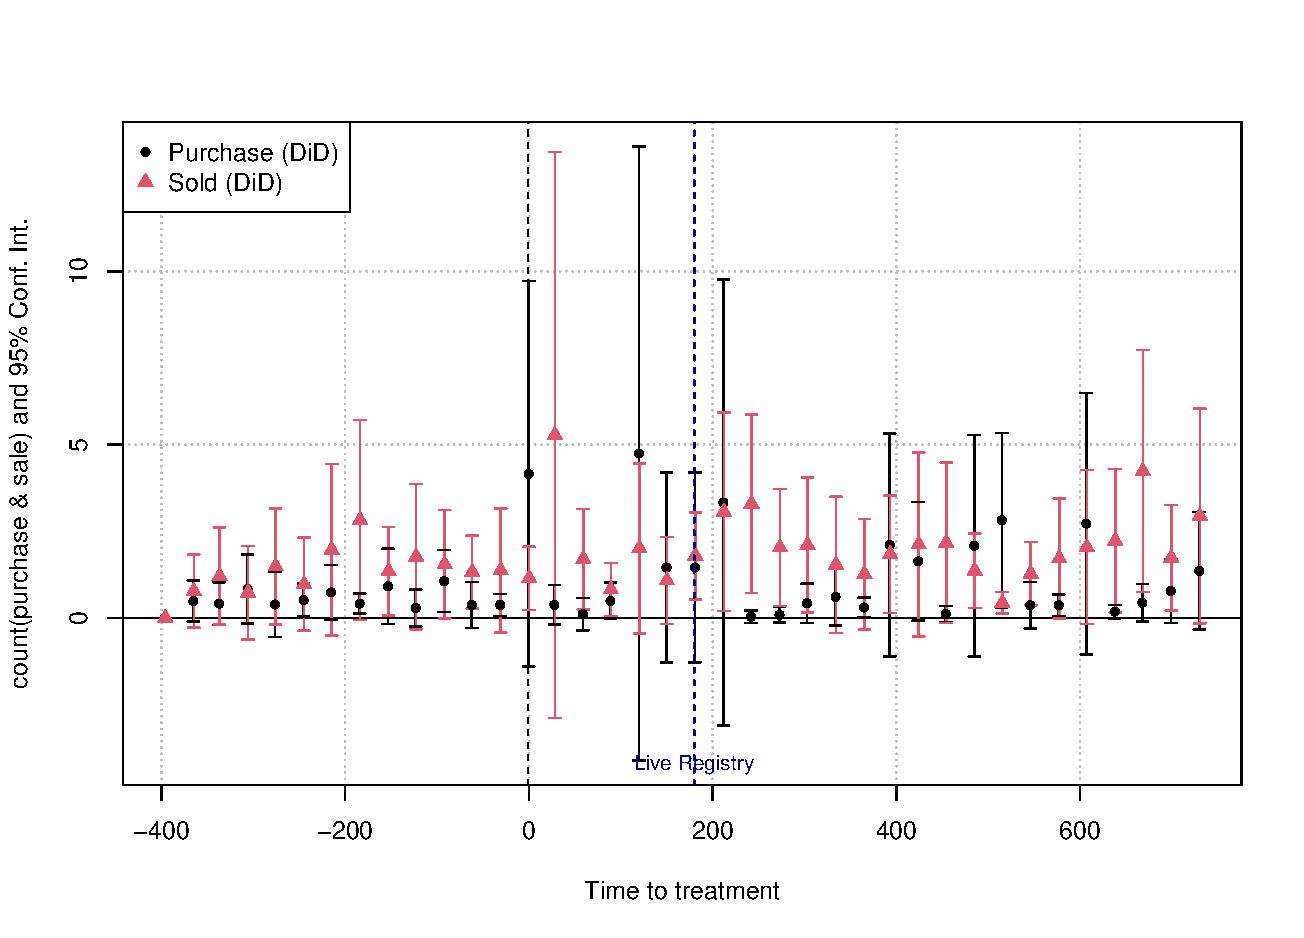
\includegraphics[width=1\linewidth]{haven_purchase.sale.pdf}
    \caption{Event-study coefficient estimates on the number of monthly purchases and sales from  all jurisdictions classified as a haven. \\ Source: (Author's Compilation)}
    \label{fig:enter-label}
\end{figure}

Considering the event studies shown in figures (7), (8) and (9), it is important to note that these event study figures plot the coefficient estimates concerning the number of purchases and sales of properties from each of the treatment groups. From Figure 7 we observe the transactional behaviour made by all havens around the treatment period and notice that before the policy was introduced the purchases of properties remained constant, relative to the property sales. However, after the re-tabling of the ECB, there is a large discrepancy initially, but the coefficient estimates become increasingly volatile. Especially when the registry goes live as there is a significant drop in the purchase of property in the month following the registries’ introduction.  Equally, the sale of property also follows a similar cyclical trend as before the treatment period, but there are larger variations in the coefficient estimates and confidence intervals after the policy announcement. Notice that before the registry goes live there appears to be anticipatory behaviour where the sale of property increases a month before the registry that continues for a short period thereafter.

\begin{figure}[H]
    \centering
    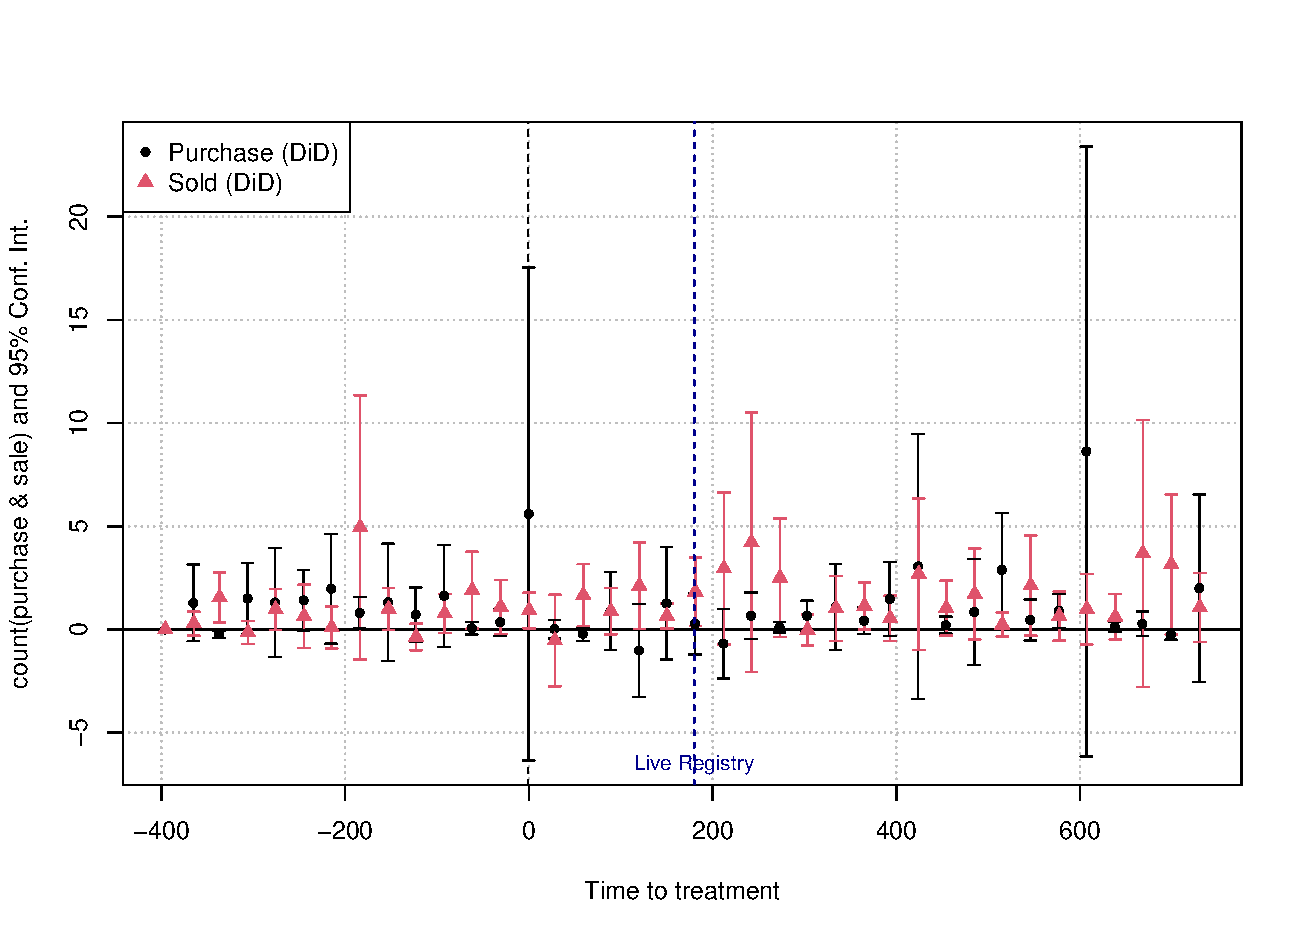
\includegraphics[width=1\linewidth]{CPI_purchase.sale.pdf}
    \caption{Event-study coefficient estimates on the number of monthly purchases and sales from havens used by corrupt countries (CPI). \\ Source: (Author's Compilation)}
    \label{fig:enter-label}
\end{figure}

Extending this to havens used by countries classified in the upper quartile of the corruption index (CPI), given in Figure (8). Before the treatment, there was a similar cyclical pattern in the transactional behaviour of these countries as seen so far. However, after the ECB was introduced, there seems to be a limited alteration in transactional behaviour. It is only a month before the registry goes live that we observe a positive trend in property sales, reaching its highest point eight months after the re-tabling of the ECB. Conversely, over the same period, the purchase of property followed an inverse relationship before the registry went live. In general, the coefficient estimates for property sales are slightly higher while purchases are marginally lower in the months around when the registry was introduced. If we consider the whole period, the results suggest a short-term effect of the policy in altering transactional behaviour in highly corrupt countries, as we later observe transactional behaviour similar to the pre-treatment levels after this eight-month period.

\begin{figure}[H]
    \centering
    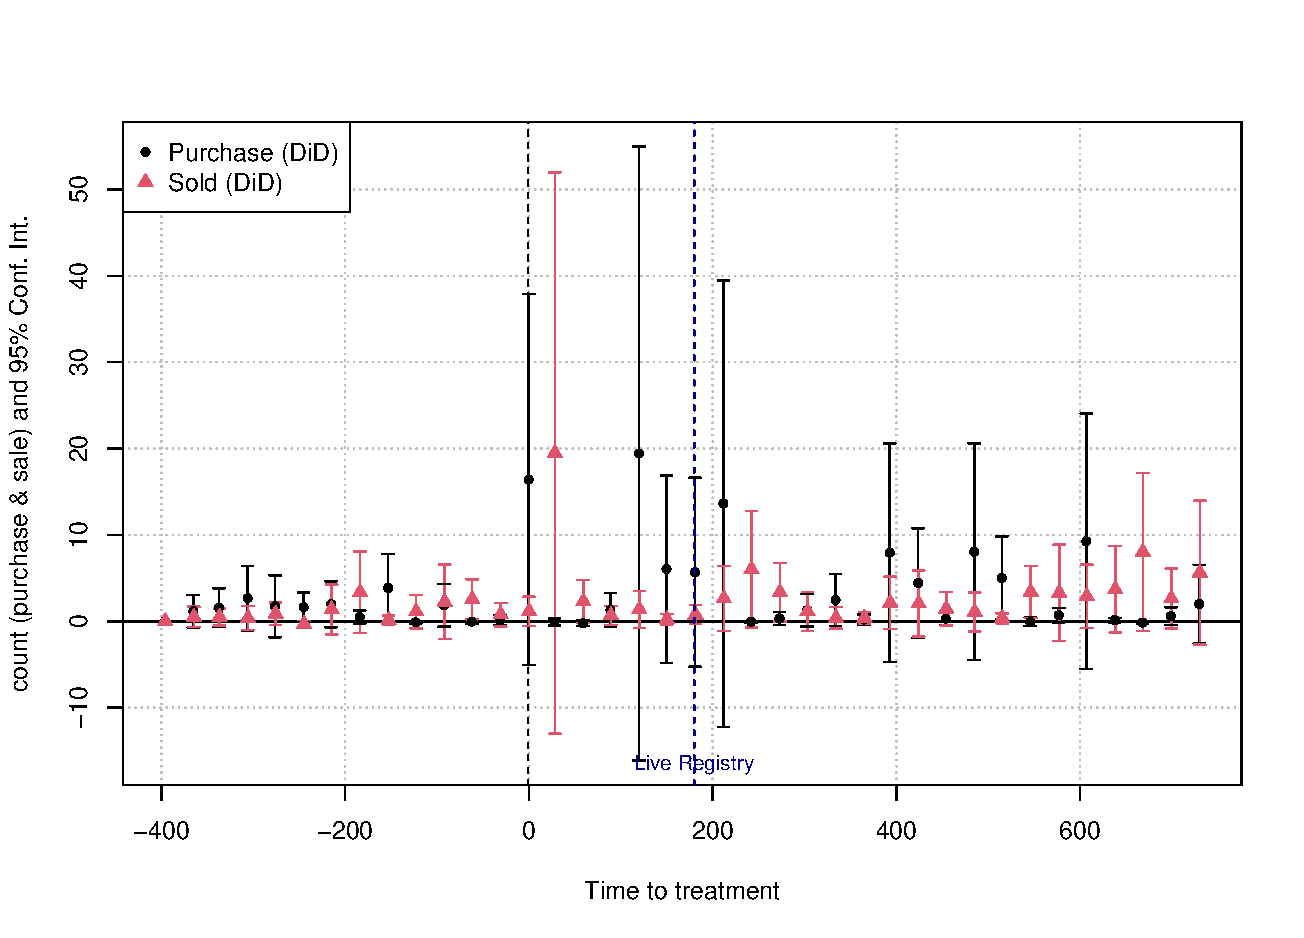
\includegraphics[width=1\linewidth]{AEOI_purchase.sale.pdf}
    \caption{Event-study coefficient estimates on the number of monthly purchases and sales from havens used by countries that are signatories to the AEOI. \\ Source: (Author's Compilation)}
    \label{fig:enter-label}
\end{figure}

Finally, Figure 9 presents the event study for countries that are signatories to the AEOI. What we observe are similar variations in the transactional behaviour from these countries that are characterised by marginal fluctuations in the purchase and sale of properties before the policy introduction. Once the policy is introduced there is an immediate discrepancy in the coefficient estimate for the purchases, and the sale a month after the ECB announcement. Given the lack of validity in the estimates initially, it does appear that there is a limited effect in the sale of property two months after the re-tabling of the ECB. However, once the registry goes live there is some evidence that there is an increasing trend in sales that is also reflected by significantly limited property purchases. Nonetheless, these apparent trends seem to be short-lived as we observe patterns similar to pre-treatment levels.

In summary, the analysis exploring the impact of increased transparency on the offshore property market reveals nuanced findings. Initial results, reflected in Table 3, show a statistically significant decline in property ownership by overseas havens as compared to non-havens, with a similar trend in highly corrupt countries. Yet, this pattern diverges for countries adhering to the Common Reporting Standard (CRS), where no deterrent effect on ownership from the Economic Crime Bill (ECB) is evident, suggesting potential non-compliance or concealment efforts in light of commitments to the Common Reporting standards. The estimates for the purchases of property present mixed results; although tax haven purchases show no significant change, there is a slight decrease in purchases by corrupt countries. Notably, there is a robust positive relationship in property transactions by Automatic Exchange of Information (AEOI) participants, with a significant 75${\%}$ increase in value alongside a 14.9${\%}$ and 42.5${\%}$ rise in sales volume and value across all havens, respectively. This is reflected by a 19.7${\%}$ and 31.6${\%}$ increase in sales by CPI and AEOI countries. Event studies, particularly Figures 7 and 9, demonstrate that while the ECB induces initial volatility, especially in property purchases among havens, the effect stabilises over time. In highly corrupt countries, a short-term spike in sales post-ECB gives way to a reversion to pre-policy transactional patterns. Similarly, AEOI signatories show immediate fluctuations post-policy, but later trends align with the differential findings, suggesting a transient policy impact. Overall, it is apparent that while the ECB influences transaction behaviours temporarily, the lasting effects appear limited when considering the broader context of the difference-in-difference estimates.

\section{Discussion}

In this paper, I attempt to measure the impact that greater transparency has had on the offshore property market. Our results show that the Economic Crime Bill has led to a decrease in offshore investments made by Russian nationals and various high-risk groups. Crucially our results support some of the previous findings in the related literature, specifically from Collin et al. (2023) working paper, which finds an effective stalling out of the UK offshore property market. However, our results deviate from this paper in that we find a marginal effect in transactional behaviour. Specially Collin et al. (2023) found a strong and significant reduction in purchases made in havens favoured by Russians as well as havens used by highly corrupt and CRS-participating countries, whereas we find evidence to suggest that property purchases by Russian-favoured havens had not decreased following the introduction of the policy, but we have limited evidence to suggest otherwise for the alternative treatment groups. In addition Collin et al. (2023) also find that this relationship does not extend to the sale of properties, concluding that the forestalling in the bill had prevented a large-scale sell-off in real estate. However, the results from this paper would suggest otherwise, finding that there is a marginal but consistent sale of properties made by Russian favoured havens in addition to all the treatment groups in our analysis. 

It is therefore important to discuss that the contrast in these findings can be partly attributed to certain methodological and empirical differences. Firstly, Collin et al. (2023) consider the effect of the ECB on a national level, whereas our scope of interest is strictly confined within The Greater London area. As there is strong evidence of deterrence following the ECB on a national level, the contrast in results could suggest regional differences in terms of the policy's effectiveness in altering transactional behaviour. Given London’s unique position and its heterogeneity to the rest of the UK, this could be evidence that a regional policy is needed. Specifically, London’s network of financial services and its opaque laws are perhaps dampening the effects of the attempts to introduce transparency within its offshore property market concerning the rest of the UK. Ultimately this could be the overriding factor that is driving the discrepancy in our results from the existing literature. 

In addition to this, I also consider an alternative empirical approach, by modelling a triple difference in difference estimation that accounts for district-level favourability in addition to the haven use, it uncovers one of the limitations of estimating true beneficial ownership that has been previously identified. This paper is also able to take advantage of the latest versions of the OCOD dataset that include property transactions up to February 2024, therefore accounting for the impact following the registry compliance deadline which was the end of January 2023. This ultimately enables us to account for certain lags in reporting title registrations to the UK authorities in our estimates which could further address certain contrasts in existing findings.

\subsection{Limitations}

It is important to acknowledge that although our estimates have some advantages, several limitations need to be discussed. Firstly, due to the complex nature of attempting to accurately measure true beneficial ownership, it is extremely challenging to categorise actual property ownership to certain demographics. In a broader sense, measuring the effects of the ECB on all havens is useful in capturing the general effect of the policy. However, the problem becomes more complicated when attempting to narrow the scope of analysis by targeting certain groups. Taking advantage of Russian behavioural traits in terms of their preference for overseas jurisdictions and districts provides a useful foundation for analysis. But the scale of illicit activity has essentially blurred the lines, making it difficult to measure true beneficial ownership accurately. A prominent example is countries such as Gibraltar and Cyprus which have a large number of Russian beneficial owners. These countries also see around 90{\%} of their investments coming from other nationals in the Middle East, Africa, and Asia.

There are also inherent limitations with the proposed methodology put forward in this paper. Specifically, the parallel trend assumption that underpins the validity of the difference in difference estimates must hold. Such that in the absence of the ECB the transactional behaviour in property from the treatment groups and control groups would have followed parallel trends over time. Equally, when adding an additional layer with regards to the triple difference in difference estimate, adds additional complexities to our assumptions. Such that we require in the absence of the policy the difference in property transactions between Russian-favoured jurisdictions and every other jurisdiction, and the difference in property transactions between Russian-favoured districts to every other district in London to follow a parallel trend over time. From Figure (2), jurisdictions favoured by Russians and all jurisdictions followed a downward trend before the policy introduction. After the policy, there does appear to be contrasting trends. The total stock from havens favoured by Russians follows a constant negative trend whereas the stock of ownership from all respective jurisdictions does not. This could be evidence to validate the parallel trend assumption. However, it is important to note that the implementation of the ECB was pushed forward in response to Russia’s invasion of Ukraine, but what also followed were a series of sanctions and asset freezing. Therefore, Oligarchical investment in the London Property market may have been significantly reduced in anticipation of political tension regarding Russian money in light of the invasion, as opposed to concerns about beneficial ownership transparency. Therefore, this factor could be driving this trend in the data which could undermine our assumptions.

Moreover, it's important to address the assumption of a static treatment effect in our simple difference-in-difference models. In the context of our discussion, we are assuming that when the ECB is introduced, its impact on our respective treatment groups remains constant in all subsequent periods. Implying a uniform effect of the treatment across time. Questions must be asked about the validity of this assumption; not only is there a lagged implementation of the policy, but as previously mentioned, there have been many concerns regarding the effectiveness of this policy, due to the loopholes that were identified. As a result, we are likely to observe a diminishing impact of the policy as individuals find ways to adapt to the attempted introduction of transparency. Therefore, we are unlikely to observe this uniform effect which could potentially undermine the validity of our baseline estimates. 
Whilst our basic difference in difference models overlook important dynamic effects, the event study versions of our models, which include the interaction between the treatment indicator and periods around the policy implementation, provide a better alternative in capturing these dynamic treatment effects. Offering valid insights into how the effects change over time.
 


\subsection{Wider Discussion}
The efforts to enhance transparency within the UK's property market have barely scratched the surface. The underlying issue is far more complex and entrenched than policy alone can address. The London property market, notorious for its role as the Laundromat for the world’s dirty money, serves as an important case study. Revealing a systemic problem deeply rooted in the societal and political foundations of the country.

The influence of kleptocracy within the UK extends far beyond the scope of the property market, embedding itself within the political and economic systems. This is not a recent nor surprising phenomenon; for decades, corrupt Russian oligarchs have established ties with the British political elite. The work of scholars like David Siegal, who delves into Russian informal politics, underscores the extensive reach of this oligarchical influence. As mentioned, Russia is built on a system where power is confined within Putin’s sphere of influence, a system that infiltrates all levels of Russian society. But what needs to be considered is that this political reach is perhaps not detained within the borders of Russia. What is instead evident is that the UK’s longstanding leniency and myopic approach to enforcing anti-corruption measures has allowed this idea of informal politics to penetrate the UK from abroad, redefining the societal norms from within our political system.

The real-world demonstrations of these issues are clear. Figures such as Lord Lebedev; son of a KGB officer who derived his fortune from a Kleptocratic system (Pickard, 2023), exemplify the complex connections of legitimate business fronts and illicit wealth, rooted in kleptocracy. These relationships have not only survived but flourished, shaping policy and economic landscapes to suit their ends towards a system of ‘Chumocracy’ (Benett, 2021). The infiltration is so rooted within the UK system, that oligarchs have been able to place their influence within the very institutions meant to safeguard against such corruption. Effectively explaining the UK government's pattern and continuation on the stalling of meaningful anti-corruption measures.

Ultimately the UK's response to the infiltration of kleptocracy has been stagnant. The crisis in Ukraine served as a wake-up call, highlighting the severity of the situation. However, legislative measures like the Economic Crime Bill, despite their promise, have fallen short of their potential. The limitations of tools such as a Registry of Beneficial Ownership and Unexplained Wealth Orders, illustrate the gap between policy intent and its execution, often hampered by inadequate enforcement mechanisms that we consistently observe and the resilient networks of oligarchic power.

Britain and in particular London is a very open and exposed financial hub, it is one of the reasons that illicit activity has been so ripe over the last few decades. However, this level of exposure puts the UK in a unique position to tackle complicity in kleptocracy. It is important to note that, whilst the US sanctions have historically failed to deter the actions of Russia (Seigal 2019), it does not necessarily mean that foreign policy built on the idea of informal politics is wrong. Fundamentally, in the context of UK sanctions, the scale of illicit activity and the ties London has with these prominent individuals, means the government could essentially inflict a greater influence. Specifically, a holistic approach is needed—one that encompasses not just stricter regulations and enforcement in London and the UK’s crown dependencies, but also a fundamental shift in political accountability. This involves not only closing the loopholes used by oligarchs but also actively dismantling the financial and political infrastructure that supports them. By leading global efforts against kleptocracy, the UK can redefine its role on the world stage.

\section{Conclusion}
In this dissertation, I explore the dynamics of London's offshore property market. Focusing on the intersection of global financial flows and local regulatory frameworks. The study analyses the enforcement of the Economic Crime Bill (ECB) of 2022 and its implications for offshore property ownership in London. This research sheds light on London's complex character. It is a city of financial significance and a haunt for clandestine wealth. This paper evaluates the ECB's implementation and the nuanced responses from various stakeholders. It highlights the significant but contested strides made to curb the flow of illicit funds into the UK's real estate sector. The Register of Overseas Entities, which is central to the ECB, is a pivotal attempt to uncover the secrecy surrounding offshore property ownership.

However, the analysis also reveals the challenges and loopholes that undermine the effectiveness of the ECB. The empirical evidence presented in this paper points to a complex landscape of compliance and circumvention. The behaviour of Russian oligarchs and other foreign investors in response to the ECB underscores the adaptive nature of illicit financial networks and the ongoing struggle to enforce transparency. This paper advocates for a nuanced understanding of beneficial ownership transparency and its impact on the integrity of the global financial system. Concluding that while legislative measures like the ECB are steps in the right direction, the path towards comprehensive transparency and accountability in the financial sector is tangled with obstacles.

The fight against illicit financial flows, particularly within property ownership, requires ongoing vigilance, adaptability, and a commitment to global collaboration. The UK's attempt, as examined through the lens of the ECB, demonstrates both the achievements and the limitations of current efforts. This work underscores the crucial for future research to investigate the effectiveness of transparency initiatives further and assess the broader socio-economic consequences of eradicating illicit wealth from the global financial system. As London embarks to disentangle itself from the notoriety of being a laundering capital, this dissertation underscores the complexities, challenges, and potential pathways that lie ahead in pursuing a more transparent and accountable global financial landscape.
\newpage

\begin{thebibliography}{x}
\bibitem{}
Alstadsæter, A., and A. Økland (2022). ‘Hidden in Plain Sight: Offshore Ownership of Norwegian Real Estate’. Mimeo.

\bibitem{}
Alstadsæter, A., G. Zucman, B. Planterose, and Økland, A. (2022). ‘Who Owns Offshore Real Estate? Evidence from Dubai’. EU Tax Observatory Working Paper. Paris: EU Tax Observatory.

\bibitem{}
Beioley, K., and L. Hughes (2022). ‘UK Set to Cap Costs for Agencies Pursuing Unexplained Wealth Orders’. Financial Times, 17 February.

\bibitem{}
Beioley, K., G. Hammond, and L. Hughes (2022). ‘What Are the Main Points of the UK’s Economic Crime Bill?’ Financial Times, 1 March.

\bibitem{}
Beer, S., M.D. Coelho, and S. Leduc (2019). ‘Hidden Treasure: The Impact of Automatic Exchange of Information on Cross-Border Tax Evasion’. Technical Report. Washington, DC: International Monetary Fund. https://doi. org/10.2139/ssrn.3524307

\bibitem{}
Bellemare M. F., C. J. Wichman (2020). Elasticities and the inverse hyperbolic sine transformation. Oxford Bulletin of Economics and Statistics. 82, 50–61.

\bibitem{}
Benett. D (2021). ‘The Conservatives and the whiff of chumocracy’. Available at: https://www.ft.com/content/9230bc88-9038-40a3-a785-14e78253ecd9 (accessed 13 March 2024)

\bibitem{}
Bethmann, D., and M. Kvasnicka (2016). ‘International Tax Evasion, State Purchases of Confidential Bank Data and Voluntary Disclosures’. Working Paper. Magdeburg: Otto-von-Guericke-University Magdeburg.

\bibitem{}
Bomare, J., and S.L.G. Herry (2022). ‘Will We Ever be Able to Track Offshore Wealth? Evidence from the Offshore Real Estate Market in the UK’. EU Tax Observatory Working Paper. Paris: EU Tax Observatory.

\bibitem{}
Borisovich, R. (2016). “Kleptocracy Tours” Expose State Failure to Stop Dirty Money Buying up London’. The Guardian, 2 March.

\bibitem{}
Bourne, J., Ingianni, A., & McKenzie, R. (2023). What’s in the laundromat? Mapping and characterising offshore-owned residential property in London. Environment and Planning B: Urban Analytics and City Science, 50(9), 2430-2451. https://doi.org/10.1177/23998083231155483

\bibitem{}
Carboni O. A. (2012). An empirical investigation of the determinants of R&D cooperation: An application of the inverse hyperbolic sine transformation. Research in Economics. 66, 131–41.

\bibitem{}
Carroll C. D., K. E. Dynan, S. D. Krane (2003). Unemployment risk and precautionary wealth: Evidence from households’ balance sheets. Review of Economics and Statistics. 85, 586–604.

\bibitem{}
Casi, E., C. Spengel, and B.M. Stage (2020). ‘Cross-Border Tax Evasion after the Common Reporting Standard: Game Over?’ Journal of Public Economics, 190: 104240. https://doi.org/10.1016/j.jpubeco.2020.104240

\bibitem{}
Collin, M. , Hollenbach, F.M., Szakonyi, D. (2023) The end of Londongrad? The impact of beneficial ownership transparency on offshore investment in UK property. WIDER Working Paper 2023/11. Helsinki: UNU-WIDER. https://doi.org/10.35188/UNU-WIDER/2023/319-2

\bibitem{}
Cvijanovic ́, D., and C. Spaenjers (2021). ‘“We’ll Always Have Paris’”: Out-Of-Country Buyers in the Housing Market’. Management Science, 67(7): 4120–38. https://doi.org/10.1287/mnsc.2020.3686

\bibitem{}
De Simone, M. (2015). Corruption on Your Doorstep: How Corrupt Capital Is Used to Buy Property in the UK. London: Transparency International UK.

\bibitem{}
Duan N., W. G. Manning, C. N. Morris, J. P. Newhouse (1983). A comparison of alternative models for the demand for medical care. Journal of Business and Economic Statistics. 1, 115–26.

\bibitem{}
Financial Times (2021) ‘The Conservatives and the whiff of chumocracy’. Available at: https://www.ft.com/content/9230bc88-9038-40a3-a785-14e78253ecd9 (accessed 22 March 2024)

\bibitem{}
Financial Times (2022). ‘How London became the dirty money capital of the world’. Available at: https://www.ft.com/video/d3bafb94-9dbd-4c1e-8016-8cd8331960f1 (accessed 13 March 2024)

\bibitem{}
Global Witness (2013). ‘The Companies We Keep: What the UK’s Open Data Register Actually Tells Us about Company Ownership’. Technical Report. London: Global Witness.

\bibitem{}
GOV.UK (2024). ‘Overseas companies that own property in England and Wales”. Available at: https://use-land-property-data.service.gov.uk/datasets/ocod (accessed November 2023). Information produced by HM Land Registry © Crown copyright [2024]

\bibitem{}
Hale, Henry E. 2015. Patronal Politics: Eurasian Regime Dynamics in Comparative Perspective. New York, NY: Cambridge University Press.

\bibitem{}
Hale, Henry E. 2017. “Russian Patronal Politics Beyond Putin,” Dædalus 146 (2): 30–40. 

\bibitem{}
Hawley, S. (2022). ‘The UK Has a Dirty Money Problem: Can the Government Fix It?’ openDemocracy, 11 May.

\bibitem{}
International Consortium of Investigative Journals (2024). “Offshore Leaks Database”. Available at: https://offshoreleaks.icij.org/ (accessed November 2023)


\bibitem{}
Knight Franck (2016). The Wealth Report 2016.

\bibitem{}
Londoño-Vélez, J., and J. Ávila-Mahecha (2021). ‘Enforcing Wealth Taxes in the Developing World: Quasi-Experimental Evidence from Colombia’. American Economic Review: Insights, 3(2): 131–48 https://doi.org/ 10.1257/aeri.20200319

\bibitem{}
Makortoff, K. (2022). ‘Government Denies Claims It Has Scrapped Crucial Economic Crimes Bill’. The Guardian, 26 January.

\bibitem{}
Menkhoff, L., and J. Miethe (2019). ‘Tax Evasion in New Disguise? Examining Tax Havens’ International Bank Deposits’. Journal of Public Economics, 176: 53–78. https://doi.org/10.1016/j.jpubeco.2019.06.003

\bibitem{}
Morgan Brennan (2013). ‘The World’s Most Expensive Billionaire Homes’. Available at: https://www.forbes.com/pictures/mhj45edfjh/kensington-palace-gardens-london-u-k-2/?sh=731a89c51962 (accessed 12 April 2024)

\bibitem{}
N’guessan Y. G., A. Featherstone, O. Odeh, S. Upendram (2017). Choice of the empirical definition of zero in the translog multiproduct cost functional form. Applied Economics Letters. 24, 1112–20.

\bibitem{}
O’Reilly, P., K.P. Ramirez, and M.A. Stemmer (2019). ‘Exchange of Information and Bank Deposits in International Financial Centres’. Working Paper. Paris: OECD.

\bibitem{}
Pickard J. (2023) ‘Boris Johnson faces fresh questions over 2018 party at Lebedev villa’. Available at: https://www.ft.com/content/53d32fbc-a1e5-495b-b068-cf7d7a202f78 (accessed 22 March 2024)

\bibitem{}
Ravallion M. (2017). A concave log-like transformation allowing non-positive values. Economics Letters. 161, 130–32.

\bibitem{}
Sá, F. (2016). The Effect of Foreign Investors on Local Housing Markets: Evidence from the UK.

\bibitem{}
Siegel, D. (2022). ‘FROM OLIGARCHS TO OLIGARCHY: The Failure of U.S. Sanctions on Russia and its Implications for Theories of Informal Politics’. World Affairs, 185(2), 249-284. https://doi.org/10.1177/00438200221094588

\bibitem{}
The Economist (2022). ‘A New Book Shows How Britain Came to Welcome Dirty Money,’ 12 March.

\bibitem{}
Transparency International UK (2022a). ‘Stats Reveal Extent of Suspect Wealth in UK Property and Britain’s Role as Global Money Laundering Hub’. Available at: https://www.transparency.org.uk/uk-money-laundering-stats-russia-suspicious-wealth (accessed 14 November 2024).

\bibitem{}
Williams, M. (2022). ‘UK May Ditch Plans to Stop Fraudsters Using Fake Names to Run Businesses’. openDemocracy, 26 January.

\bibitem{}
William Wallis (2023) ‘Russian oligarchs used ‘golden visa’ scheme to settle in UK’. Available at: https://www.ft.com/content/be98a66a-f595-47f9-b088-2c2368d11d19 (accessed 13 March 2024).


\end{thebibliography}

\appendix
\section{Robustness Results}
\subsection{Russian Re-specification}
\begin{table}[H]
\caption{Difference-in-difference and Triple Difference-in-difference estimation of transactions from Jurisdictions favoured by Russians}
\label{yourLabelHere}
\centering
\large 
\begin{adjustbox}{width=1.25\textwidth,center}
\begin{threeparttable}
\begin{tabular}{@{}lccccccccc@{}}
\hline
\hline \\ [-1.8ex]
 & \multicolumn{3}{c}{Stock} & \multicolumn{3}{c}{Purchase} & \multicolumn{3}{c}{Sale} \\
\cmidrule{2-4} \cmidrule{5-7} \cmidrule{8-10}
& Stock & ihs(Stock) & ihs(£Volume) & Purchase & ihs(Purchase) & ihs(£Volume) & Sale & ihs(Sale) & ihs(£Volume) \\
\hline \\[-1.8ex]
Russia $\times$ Post & $-$35.135$^{***}$ & $-$0.022 & -0.0618 & $-$0.011 & $-$0.044 & 0.005 & 0.469 & 0.368$^{***}$ & 0.980 \\
& (5.954) & (0.025) &  (0.147) & (0.699) & (0.077)& (0.778) & (0.547) & (0.084) & (0.732) \\
\hline \\ [-1.8ex]
Observations & 6,779 & 6,779 & 6,779 & 6,591 & 6,591 & 6,591 & 6,591 & 6,591 & 6,591 \\
\hline
\hline \\ [-1.8ex]
Russia$\times$Post$\times$District &  1.280 & 0.007 & 0.445 & 0.015 & -0.008 & 0.935** & 0.042& 0.055* & 1.44$^{***}$ \\
& (15.310) & ( 0.106) & (0.694) & (0.091) & (0.019) & (0.342) & (0.107) & (0.030) & (0.325)\\
\hline \\ [-1.8ex]
Observations & 56,665 & 56,665 & 56,665 & 56,665 & 56,665 & 56,665 & 56,665 & 56,665 & 56,665 \\
\hline
\hline \\ [-1.8ex]
\end{tabular}
\begin{tablenotes}
\item
    Note: This table presents the difference-in-difference estimates and the triple difference-in-difference estimates of the total stock, purchase and sale of London property by offshore companies situated in overseas jurisdictions in the upper quartile of havens in the Russian column given in Figure (1). Also included are the inverse hyperbolic sine transformation of each of the dependent variables respectively. (i) The treatment group are havens favoured by Russians and all other overseas jurisdictions as the control groups. (ii) The treatment groups are havens favoured by Russians and London districts favoured by Russians that are idenitifed by Bomare and Herry (2022), and all other overseas jurisdictions and London districts acting as the control. Standard errors are clustered at the overseas jurisdiction level. $^{*}$p$<$0.1; $^{**}$p$<$0.05; $^{***}$p$<$0.01
\end{tablenotes}
\end{threeparttable}
\end{adjustbox}
\end{table}


\begin{figure}[H]
    \centering
    \begin{subfigure}[b]{0.8\textwidth}
        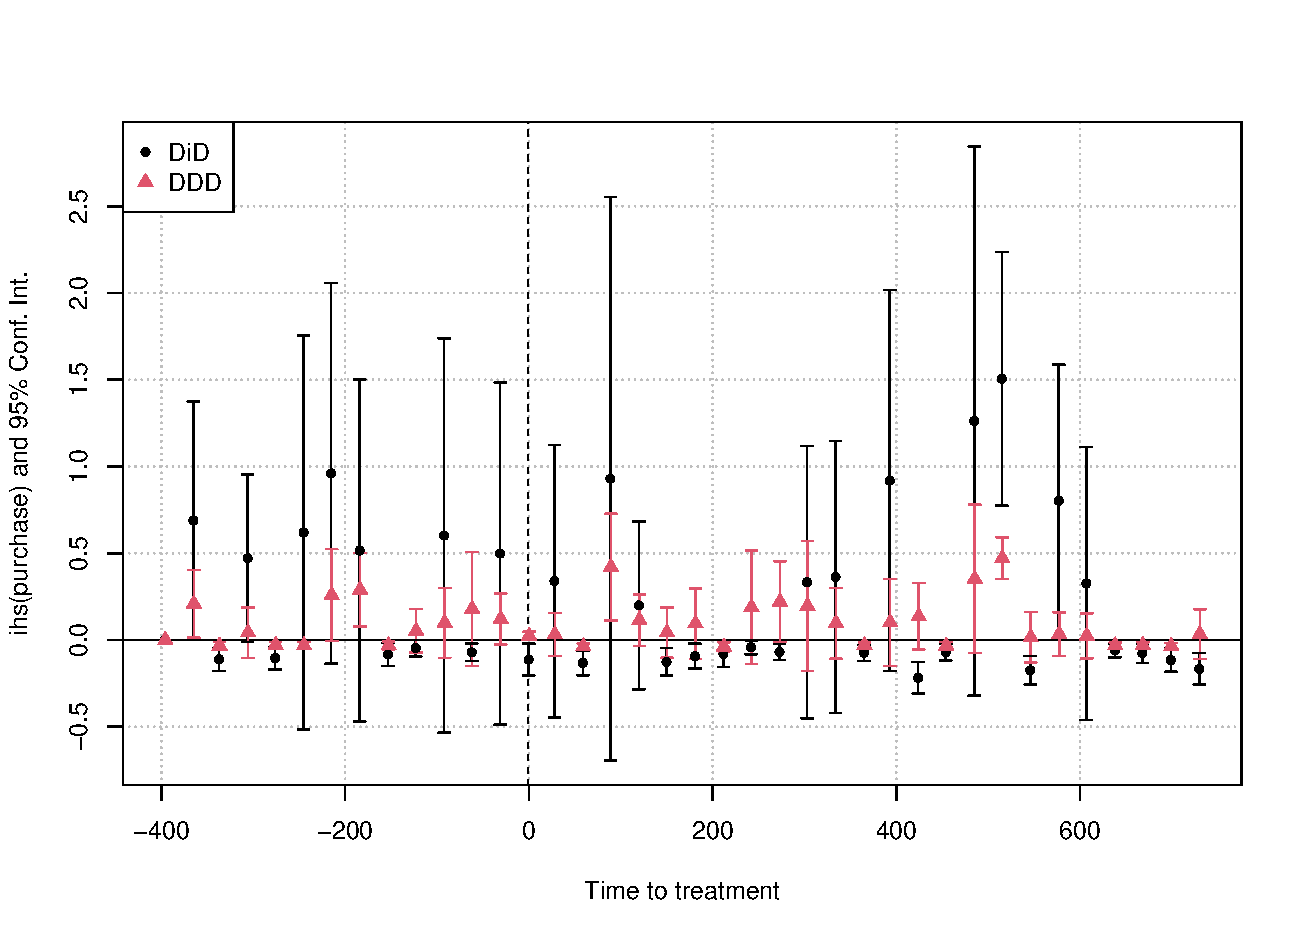
\includegraphics[width=\textwidth]{Event_study_Purchase_Russia_Robust.pdf}
        \caption{Difference-in-difference (DiD) and Triple difference-in-difference (DDD) specification coefficient estimates on monthly property purchases from re-classified Russian favoured overseas jurisdictions.}
        \label{fig:purchase-event}
    \end{subfigure}
    
    % Add some vertical space between the figures, if desired
    \vspace{1cm}
    
    \begin{subfigure}[b]{0.8\textwidth}
        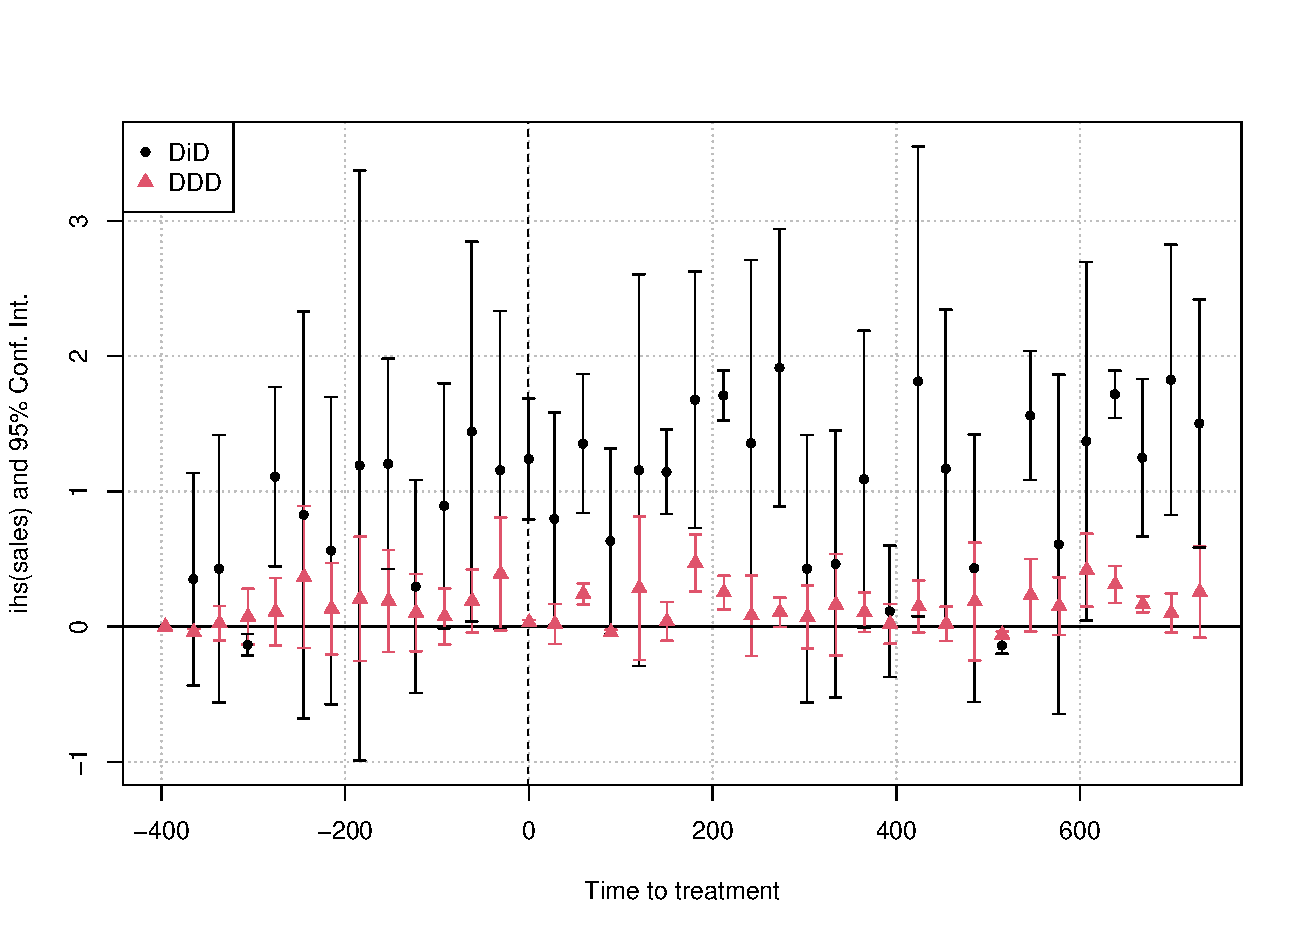
\includegraphics[width=\textwidth]{Event_study_Sale_Russia_Robust.pdf}
        \caption{Difference-in-difference (DiD) and Triple difference-in-difference (DDD) specification coefficient estimates on monthly property sales from re-classified Russian favoured overseas jurisdictions.}
        \label{fig:sale-event}
    \end{subfigure}
    \caption{Event study coefficient estimates on the inverse hyperbolic sine transformation of monthly property purchases and sales made by companies registered in re-classified Russian favoured tax havens.  Source: (Author's Compilation).}
    \label{fig:overall-event}
\end{figure}

\subsection{Alternative Treatment Groups Re-specification}
\begin{table}[H]
\caption{Difference-in-difference and Triple Difference-in-difference estimation of transactions from Jurisdictions favoured by Russians}
\label{yourLabelHere}
\centering
\large % Adjust font size as needed
  \begin{adjustbox}{width=1.25\textwidth,center}
\begin{threeparttable}
    \begin{tabular}{@{}lccccccccc@{}}
\toprule
 & \multicolumn{3}{c}{Stock} & \multicolumn{3}{c}{Purchase} & \multicolumn{3}{c}{Sale} \\
\cmidrule{2-4} \cmidrule{5-7} \cmidrule{8-10}
& Stock & ihs(Stock) & ihs(£Volume) & Purchase & ihs(Purchase) & ihs(£Volume) & Sale & ihs(Sale) & ihs(£Volume) \\
\midrule
CPI$\times$POST & $-$16.398$^{***}$ & $-$0.033 & $-$0.037 & $-$0.126 & $-$0.028 & 0.639 & 0.214 & 0.163$^{*}$ & -0.109 \\
 & (5.967) & (0.025) & (0.082) & (0.700) & (0.077) & (0.435) & (0.547) & (0.084) & (0.732)\\
\midrule
AEOI-signatories$\times$POST & 14.588$^{**}$ & $-$0.043$^{*}$ & $-$0.046 & $-$0.665 & $-$0.118 & 0.749$^{*}$ & 0.316$^{***} & $ 0.371$^{***}$ & 0.096 \\ 
& (5.968) & (0.025) & (0.082) & (0.700) & (0.077)  & (0.435) & (0.047) & (0.084) & (0.409) \\
\midrule
Observations & 56,665 & 56,665 & 56,665 & 56,665 & 56,665 & 56,665 & 56,665 & 56,665 & 56,665 \\
\midrule
\end{tabular}
\begin{tablenotes}
    \item Note: This table presents the difference-in-difference estimates of the total stock, purchase and sale of London property by offshore companies situated in overseas jurisdictions as previously defined. The measurement for analysis is an overseas jurisdiction, with a treatment period of February 2022 (The Month of the Russian invasion of Ukraine and the re-tabling of the ECB). (i) The treatment group are countries that fall in the bottom quartile of Transparency International's Corruption Perceptions Index that follow a re-classification of havens. (ii) The re-classification of havens that are most favoured by countries that are from CRS/AEOI participating countries. Standard errors are clustered at the overseas jurisdiction level.    $^{*}$p$<$0.1; $^{**}$p$<$0.05; $^{***}$p$<$0.01
\end{tablenotes}
\end{threeparttable}
\end{adjustbox}
\end{table}

\begin{figure}[H]
    \centering
    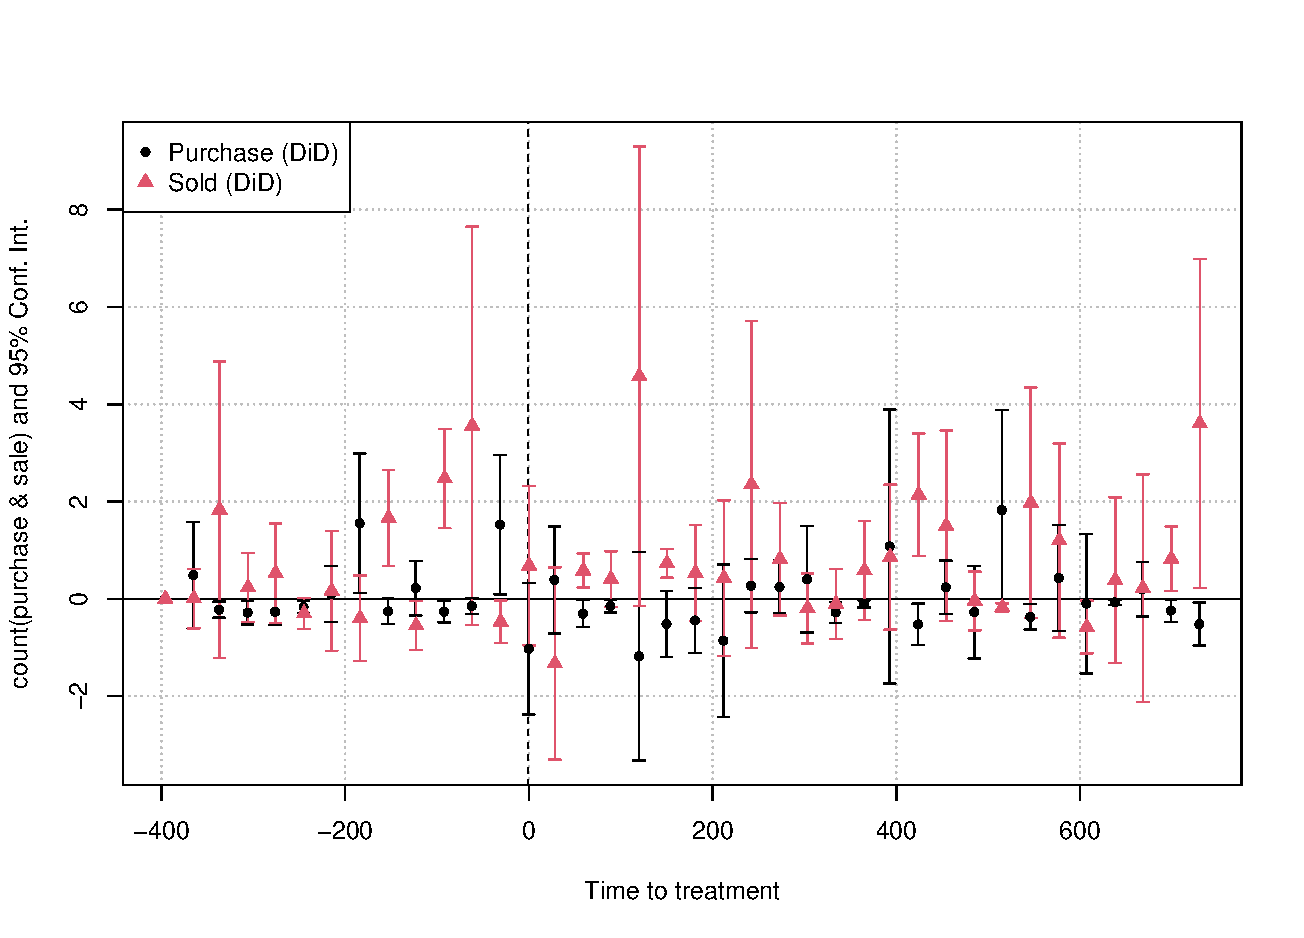
\includegraphics[width=\textwidth]{Event_study_CPI_robust.pdf}
    \caption{Event-study coefficient estimates on the number of monthly purchases and sales from re-specified havens used by corrupt countries (CPI). \\ Source: (Author's Compilation)}
    \label{fig:enter-label}
\end{figure}
\begin{figure}[H]
    \centering
    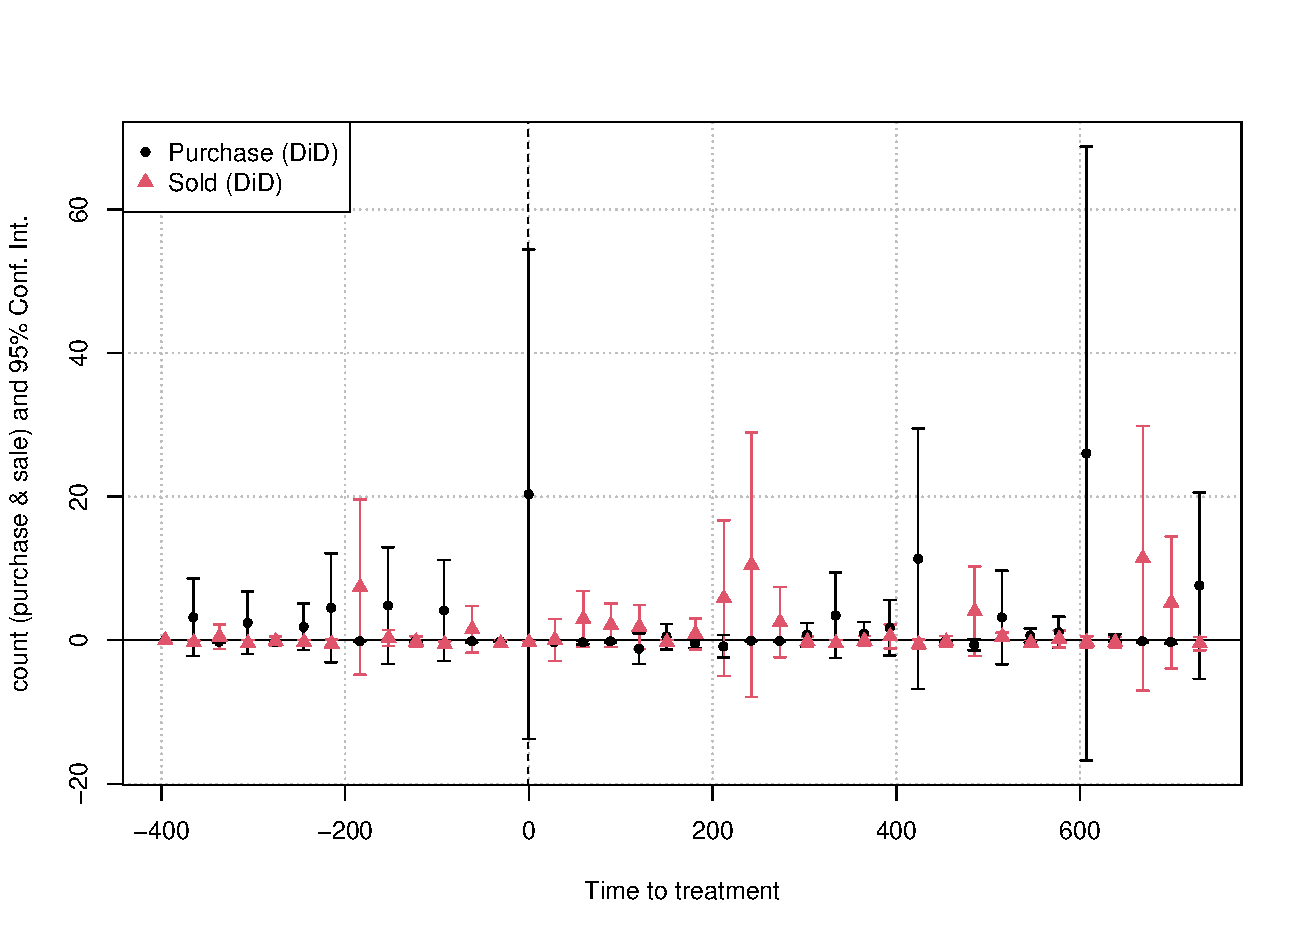
\includegraphics[width=0.9\textwidth]{Event_study_AEOI_Robust.pdf}
    \caption{Event-study coefficient estimates on the number of monthly purchases and sales from re-specified havens used by countries that are signatories to the AEOI. \\ Source: (Author's Compilation)}
    \label{fig:enter-label}
\end{figure}

\section{Lists of Havens Used}

\begin{table}[H]
\centering
\noindent
\begin{adjustbox}{width=0.9\textwidth}
\begin{threeparttable}
\begin{tabular}{lcccc}
\hline
\textbf{Country} & \textbf{Popular w/ Russians} & \textbf{CPI 25th perc.} & \textbf{CPI 50th perc.} & \textbf{AEOI signatories} \\
\hline
Anguilla  &  &  &  & x\\
Bahamas & x & x & x & \\
Belize & x & x & x & x \\
British Virgin Islands  & x &  &  & \\
Costa Rica  &  &  &  & x\\
Cyprus & x & x & x & x \\
Gibraltar & x & x & x & \\
Grenada &  &  &  & x \\
Guernsey &  & x & x & x \\
Hong Kong SAR China & x & x & x & \\
Isle of Man &  &  &  & x \\
Jersey & x &  &  & x \\
Labuan  & x &  &  &  \\
Malta  &  & x & x & \\
Mauritius  & x & x & x &  \\
Saint Kitts and Nevis  &  & x &  &  \\
Seychelles  & x &  &  & \\
Turks and Caicos Islands &  &  &  & x \\
\hline
\end{tabular}
\begin{tablenotes}
    \item Note: This table contains the list of tax havens used for each of the treatment groups in the analysis. The Russian list contains the havens where a large proportion of beneficial owners of shell companies identified in the Offshore Leaks were Russian. The CPI 25th and CPI 50th lists contain the havens where a significant proportion of beneficial owners of shell companies come from countries that are listed in the 25th or 50th percentile of most corrupt countries as defined by Transparancy Internationals Corruption Perception Index. The AEOI list contains the havens where a large proportion of beneficial owners of shell companies come from countries that are signatories to the OECD's Common Reporting Standard (CRS). 
\end{tablenotes}
\end{threeparttable}
\end{adjustbox}
\caption{Tax havens used for each of the Treatment groups}
\label{tab:your_label_here}
\end{table}

\begin{table}[H]
\centering
\begin{adjustbox}{width=0.9\textwidth}
\begin{threeparttable}
    \hspace*{-1cm} 
\begin{tabular}{lccc}
\hline
\textbf{Country} & \textbf{Consensus list} & \textbf{Menkhoff and Miethe (2019)} & \textbf{Wier et al. (2022)} \\
\hline
Andorra &  & x & x \\
Anguilla &  & x & x \\
Antigua and Barbuda & x & x & x \\
Aruba &  & x & x \\
Austria & x &  &  \\
Bahamas & x & x & x \\
Bahrain &  & x &  \\
Barbados & x & x & x \\
Belgium &  & x &  \\
Belize & x &  & x \\
Bermuda & x & x & x \\
British Virgin Islands & x & x & x \\
Cayman Islands & x & x & x \\
Chile &  & x &  \\
Cook Islands &  & x &  \\
Costa Rica &  &  & x \\
Curacao &  & x & x \\
Cyprus & x & x & x \\
Dominica &  & x & x \\
Gibraltar & x & x & x \\
Grenada &  & x &  \\
Guernsey & x & x & x \\
Hong Kong SAR China & x & x & x \\
Ireland &  & x & x \\
Isle of Man & x & x & x \\
Jersey & x & x & x \\
Jordan &  & x &  \\
Lebanon &  & x &  \\
Liberia & x & x & x \\
Liechtenstein & x &  & x \\
Luxembourg & x & x & x \\
Macao SAR China &  & x & x \\
Malaysia &  & x &  \\
Maldives &  &  & x \\
Malta & x & x & x \\
Marshall Islands &  & x &  \\
Mauritius & x & x & x \\
Monaco &  & x &  \\
Montserrat &  & x &  \\
Nauru &  & x &  \\
Netherlands Antilles &  & x & x \\
Niue &  & x &  \\
Panama & x & x & x \\
Samoa &  &  & x \\
San Marino &  & x &  \\
Seychelles & x & x & x \\
Singapore & x & x & x \\
Sint Maarten &  & x &  \\
St. Kitts and Nevis & x & x & x \\
St. Lucia & x & x & x \\
St. Vincent and Grenadines &  & x &  \\
Switzerland & x & x & x \\
Tonga &  & x &  \\
Trinidad and Tobago &  & x &  \\
Turks and Caicos Islands &  &  & x \\
U.S. Virgin Islands & x & x & x \\
Uruguay &  & x &  \\
Vanuatu & x & x & x \\
\hline
\end{tabular}
\begin{tablenotes}
    \item Note: This table illustrates the list of tax havens used in the analysis. The Consensus list contains the countries formulated by Menkhoff and Miethe (2019) that appear most often in studies of tax evasion. The Menkhoff and Miethe (2019) list contains the countries classified as tax havens in their analysis. The Wier et al (2022) list contains the countries used in their analysis (Collin, Hollenback and Szakonyi's 2023).
\end{tablenotes}
\end{threeparttable}
\end{adjustbox}
\caption{List of various havens used in studies of tax evasion}
\label{tab:jurisdictions}
\end{table}





\end{document}